\chapter{Propuesta de solución}

%=========================================================
%                                                         Problematica
%=========================================================
\section{Objetivos}
\noindent En esta sección se menciona el objetivo general y los objetivos especifícos, los cuales ayudarán a atacar la problemática.
\subsection{Objetivo General}
\noindent Desarrollar una aplicación web de apoyo para el Departamento Deportivo de la Escuela Superior de Cómputo (ESCOM) que permita la inscripción de interpolitécnicos, visualizar los eventos próximos y a su vez sea un espacio de información y difusión.
\subsection{Objetivos Especificos}
\begin{itemize}
	\item Implementar un mecanismo de validación del estatus académico del alumno. 
	\item Implementar un módulo para la generación de la cédula de inscripción con base en el formato oficial de interpolitécnicos deportivos. 
	\item Implementar un módulo de comunicación con la red social (Facebook). 
	\item Implementar un módulo de consulta de resultados de competencias.
\end{itemize}

	%=========================================================
	%                                                         Marco teorico
	%=========================================================
	
	\noindent Dentro del Instituto Politécnico Nacional (IPN) se han creado eventos que fomentan la participación y competitividad de la comunidad, llamados interpolitécnicos. Estos involucran áreas tales como: actividades deportivas, culturales o académicas, dichos eventos son de participación gratuita y se realizan 2 veces al año entre todos los planteles académicos que constituyen al IPN, divididas en los niveles Medio Superior y Superior.  \cite{Reglas}\\
	\noindent El IPN cuenta con 26 actividades deportivas registradas, sin embargo, en las unidades académicas no se practican todas.\cite{Reglas}.
	\noindent La entidad dedicada a la coordinación de las actividades deportivas con las que cuenta el IIPN, es la Dirección de Desarrollo y Fomento Deportivo \cite{DDYFD}. Esta se encarga de la creación, administración y control de todas las actividades deportivas prácticadas dentro del IPN tales como: definir el área donde se practican y la asignación de presupuesto de cada actividad deportiva, llevar un registro de la cantidad de población que practica un deporte. \cite{Reglamento}.	
	\noindent A su vez coordinan la realización de los eventos Interpolitécnicos Deportivos del IPN siguiendo ‘el reglamento general liga interpolitécnica. \cite{Reglamento}, donde se explican los  procesos que realiza cada persona involucrada.\\
	
	\noindent El Coordinador de Área Deportiva de cada Unidad Académica es el responsable de supervisar los aspectos operativos y técnicos de todos los deportes que se practican dentro de la misma así mismo es el encargado de realizar el proceso de inscripción a un interpolitécnico para los alumnos que así lo deseen y para que puedan participar este deberá solicitar la documentación de inscripción (cédula de inscripción) individual o de sus equipos y entregarlos a los Coordinadores de cada Disciplina Deportiva en la Dirección de Desarrollo y Fomento Deportivo. \cite{Reglamento} \\
	\noindent  El alumno que desee participar en un evento interpolitécno deberá acudir con el coordinador de su unidad académica para comenzar el proceso de inscripción a un evento interpolitécnico. 
	\\El coordinador le solicitará una forma para comprobar su estatus académico, este puede variar dependiendo de los coordinadores de las distintas unidades académicas. A su vez el alumno llenará el formato de inscripción al evento de su interés, anexando una fotografía. 
	\\ Si se comprueba que el alumno está inscrito en el periodo actual en el que quiere participar, podrá continuar con el proceso, en caso contrario se negará la inscripción. \cite{Reglamento}
	\\ Al concluir con la comprobación de inscripción, se le notifica al alumno cual es el estatus de su solicitud. 
	
	\noindent Para más detalles puede consultarse en el apartado Anexos Apartado \ref{ProcesoInscripcionActual}
	\pagebreak
	
	
	
	%=========================================================
	%                                                         Analisis de factibilidad tecnica
	%=========================================================
	\section{An\'alisis de Entornos de Desarrollo Interactivo}
	\noindent Éste análisis tiene como objetivo describir las herramientas que pueden ocuparse para la realización de este proyecto mencionando sus objetivos de cada herramienta de trabajo seleccionada.
	
	%=========================================================
	%                                                         IDE
	%=========================================================
	\subsection{IDE}
	\begin{itemize}
		\item  Netbeans 
		\label{Herramientas}
		\newline
		Netbeans es un entorno integrado de desarrollo o IDE (IntegratedDevelopmentEnvironment), cone el que se puede realizar todas las tareas asociadas a la programación.
		\newline
		Simplifica alguna de las tareas que, sobretodo en proyectos grandes, son laboriosas. Ofrece la posibilidad de asistencia (parcialmente) en la escritura de código, aunque no nos libera de aprender el lenguaje de programación.
		Nos ayuda en la navegación de las clases predefinidas.
		Aunque puede ser costoso su aprendizaje, los beneficios superan las dificultades.
		
	\subsection{Framework}
		\item Spring MVC \\ 
		Spring Mvc es una alternativa de framework basado en el patrón modelo-vista-controlador, después de haber aprendido de errores de frameowrks como Jakarta Struts y otras alternativas.
		El framework tiene un conjunto de interfaces que después se implementan para proporcionar la funcionalidad correspondiente. Las interfaces están acopladas claramente al Servlet Api.\cite{spring}\\
		La clase DispatcherServlet está en el front controller y es responsable de delegar y coordinar el control entre varias interfaces en la fase de ejecución durante una petición Http.
		Las interfaces más importantes definidas en Spring Mvc, y sus responsabilidades, son las siguientes:
		\begin{itemize}
			\item HandlerMapping: permite manejar peticiones de entrada.
			\item HandlerAdapter: ejecución de objetos que permiten manejar las peticiones entrantes.
			\item Controller: está entre el modelo y la vista, y permite manejar peticiones entrantes y redirigirlas a la respuesta adecuada. 
			\item Vista: responsable de retornar una respuesta al cliente. 
			\item ViewResolver: selecciona una vista basada en un nombre lógico de la vista.
			\item HandlerInterceptor: intercepta las peticiones entrantes, es comparable pero no igual a los filtros de Servlet.
			\item LocaleResolver: resuelve y opcionalmente salva el locale de un usuario individual.
			\item MultipartResolver: facilita trabajar con ficheros de subida wrapping peticiones de entrada.
		\end{itemize}
		Cada interfaz de estrategia tiene su responsabilidad importante dentro del framework general. Estas abstracciones ofrecidas por estas interfaces son potentes, pues permiten configurar un conjunto de interfaces juntas y ofrecen un conjunto en el top del Api de Servlet. Sin embargo, los desarrolladores y los vendedores son libres es escribir otras implementaciones. Spring MVC utiliza la interfaz java.util.Map como una abstracción del modelo cuando se espera que las llaves tenga valores de String. \\
		Cada testeo de las implementaciones de estas interfaces tiene otra ventaja importante dentro del alto nivel de abstracción ofrecido por Spring Mvc. Dispatcher Servlet está altamente acoplado con el contenedor de Inversión de Control de Spring para configurar las capas de web de las aplicaciones. Sin embargo, las aplicaciones web pueden utilizar otras partes del framework de Spring, incluyendo el contenedor, y decidir no usar Spring Mvc. \cite{MVC}\\
		Struts es un framework mucho más antiguo, por lo que Spring ha aprendido de la experiencia adquirida de usar Struts para no cometer los mismos errores. \cite{introspring}
		A continuación se enumeran un conjunto de ventajas:
		\begin{itemize}
			\item Spring MVC ofrece una división limpia entre Controllers, Models (JavaBeans) y Views. 
			\item Spring MVC es muy flexible, ya que implementa toda su estructura mediante interfaces, no como Struts que obliga a heredar de clases concretas tanto en sus Actions como en sus Forms. 
			\item Spring MVC provee interceptores y controllers que permiten interpretar y adaptar el comportamiento común en el manejo de múltiples requests.
			\item Los controllers de Spring MVC se configuran mediante IoC como los demás objetos, lo cual los hace fácilmente testeables e integrables con otros objetos que estén en el contexto de Spring, y por tanto sean manejables por éste. 
			\item Las partes de Spring MVC son más fácilmente testeables que las de Struts, debido a que evita la herencia de una clase de manera forzosa y una dependencia directa en el controller del servlet que despacha las peticiones. 
			\item No existen ActionForms, se enlaza directamente con los beans de negocio. 
			\item Struts obliga a extender la clase Action, mientras que Spring MVC no, aunque proporciona una serie de implementaciones de Controllers para que el usuario los utilice. Existe una gran variedad de Controladores.
			\item Spring tiene una interfaz bien definida para la capa de negocio. 
			\item Spring ofrece mejor integración con tecnologías distintas a JSP, como Velocity,XSLT,FreeMaker y XL. 
		\end{itemize}
		Las ventajas que se tiene usar Spring MVC 
		\begin{itemize}
			\item Se ha introduce un nombre es espacio MVC que simplifica la configuración.
			\item Se han insertado anotaciones adicionales como @CookieValue (permite relacionar un atributo de un método a una cookie) y @RequestMappings (asociar directamente en la clase la posibilidad de asociar una petición Url a un controlador específico).
			\item El tipo ConversionService es una alternativa más simple y robusta que los PropertyEditors de JavaBeans.
			\item Se soporta un formateo de números con el atributo @NumberFormat.
			\item Se soportan el formateo de fechas, calendarios y joda time con el atributo @DatetimeFormat, siempre que la librería Joda Time esté dentro del classpath.
			\item Se soporta la validación para entradas @Controller con la etiqueta @Valid, si se proporciona una implementación de la Jsr-303 en el classpath.
			\item Soporte para leer y escribir Xml, si Jaxb está dentro del classpath.
			\item Soporte para leer y escribir Json, si Jackson está dentor del classpath.
		\end{itemize}
		Para poder crear los controladores debemos de seguir los siguientes pasos:
		\begin{itemize}
			\item Definir una clase que implementa la interfaz del controlador.
			\item Insertar dicha clase como un objeto en el contexto de Spring.
			\item Asignar el nombre a una Uri que posteriormente será invocada por el usuario.
			\item Especificar la extensión de la uti en el DispatcherServlet de Spring, configurado en web.xml, para que se pueda buscar internamente.
		\end{itemize}
		
		El modelo son los datos con los que interactúa la vista y el controlador. En este caso, el modelo se pasa mediante un atributo de la clase ModelAndView, para posteriormente acceder al mismo desde la parte de la vista. \cite{introspring}
		
		Algunas recomendaciones para desarrollar usando Spring MVC
		Primero: determinar el Ide de desarrollo que se quiera utilizar. Existan varias alternativas: Netbeans, Eclipse, Intellij, Spring Tool Suite. Yo, por precio (gratis) y facilidad de uso (está orientado al desarrollo de Spring) recomiendo el uso de Spring Tool Suite. \\
		
		Segundo: crear el proyecto básico, y elegir nuestra herramienta de gestión de librerías. Para crear el proyecto, tenemos varias alternativas, desde configurar nosotros desde cero el servlet de spring, como utilizar plantillas ya existentes. También existe la posibilidad de descargar las librerías de la web de Spring o bien utilizar repositorios de Maven.\\
		
		Tercero: escoger el tipo de vista que se utilizará para el proyecto. En mi caso, la vista que suelo utilizar y con la que me siento más acostumbrado es Jsp.\\
		
		Cuarto: desarrollar la parte de negocio (controladores) y persistencia (seleccionando un framework como hibernate o jpa), y relacionar los controladores, con la vista y la persistencia.
		En principio, eso es todo.\\
		El framework fue lanzado inicialmente bajo Apache 2.0 License en junio de 2003. Esta licencia es una licencia de software libre creada por la Apache Software Foundation que requiere la conservación del aviso de copyright y disclaimer, pero no es una liencia copyleft, ya que no requiere la redistribución del código fuente cuando se distribuyen versiones modificadas. \cite{introspring} \\
		
		\item Facebook Developers 
		La Plataforma de Facebook es el conjunto de servicios, herramientas y productos proporcionados por el servicio de redes sociales Facebook para que los desarrolladores externos creen sus propias aplicaciones y servicios que acceden a datos en Facebook.\\
		
		La actual Plataforma de Facebook se lanzó en 2010. La plataforma ofrece un conjunto de interfaces y herramientas de programación que permiten a los desarrolladores integrarse con el "gráfico social" abierto de relaciones personales y otras cosas como canciones, lugares y páginas de Facebook. La asignación en facebook.com, sitios web externos y dispositivos pueden acceder al gráfico. \\
		
		Facebook lanzó la Plataforma de Facebook el 24 de mayo de 2007, proporcionando un marco para que los desarrolladores de software creen aplicaciones que interactúen con las funciones principales de Facebook. Se introdujo un lenguaje de marcado llamado Facebook Markup Language simultáneamente; se utiliza para personalizar el "aspecto y la sensación" de las aplicaciones que crean los desarrolladores. Usando la Plataforma, Facebook lanzó varias aplicaciones nuevas, incluyendo Regalos, permitiendo a los usuarios enviarse regalos virtuales entre sí, Marketplace, permitiendo a los usuarios publicar anuncios clasificados gratuitos, eventos de Facebook, brindando a los usuarios un método para informar a sus amigos sobre los próximos eventos, Video, Permitir a los usuarios compartir videos caseros entre ellos y juegos de redes sociales, donde los usuarios pueden usar sus conexiones con amigos para ayudarlos a avanzar en los juegos que están jugando. Muchos de los primeros juegos populares de redes sociales combinarían capacidades. Por ejemplo, uno de los primeros juegos en llegar al primer lugar de aplicación, (Lil) Green Patch, combina regalos virtuales con notificaciones de eventos a amigos y contribuciones a organizaciones benéficas a través de causas. \\
		
		Componentes de plataforma de alto nivel
		API de gráficos\\
		Graph API es el núcleo de la plataforma de Facebook, lo que permite a los desarrolladores leer y escribir datos en Facebook. Graph API presenta una vista simple y coherente del gráfico social de Facebook, que representa de manera uniforme los objetos en el gráfico (por ejemplo, personas, fotos, eventos y páginas) y las conexiones entre ellos (por ejemplo, relaciones de amigos, contenido compartido y etiquetas de fotos )\\
		
		Autenticación\\
		La autenticación de Facebook permite que las aplicaciones de los desarrolladores interactúen con la API Graph en nombre de los usuarios de Facebook, y proporciona un mecanismo de inicio de sesión único en aplicaciones web, móviles y de escritorio.\\
		
		Complementos sociales\\
		Los complementos sociales, incluidos el botón Me gusta, las recomendaciones y el feed de actividades, permiten a los desarrolladores proporcionar experiencias sociales a sus usuarios con solo unas pocas líneas de HTML. Todos los complementos sociales son extensiones de Facebook y están diseñados para que no se compartan datos de los usuarios con los sitios en los que aparecen. Por otro lado, los complementos sociales permiten a Facebook rastrear los hábitos de navegación de sus usuarios a través de cualquier sitio que cuente con los complementos. Y los datos recopilados de los hábitos de navegación de los usuarios ayudan a los vendedores y anunciantes en Facebook a dirigirse a su audiencia.\\
		
		iframes\\
		Facebook usa iframes para permitir que los desarrolladores externos creen aplicaciones que están alojadas por separado de Facebook, pero operan dentro de una sesión de Facebook y se accede a través del perfil de un usuario. Dado que los iframes esencialmente anidan sitios web independientes dentro de una sesión de Facebook, su contenido es distinto del formato de Facebook. \\
		
		Originalmente, Facebook utilizaba el 'Lenguaje de marcado de Facebook (FBML)' para permitir a los desarrolladores de aplicaciones de Facebook personalizar el "aspecto y la sensación" de sus aplicaciones, hasta cierto punto. FBML es una especificación de cómo codificar contenido para que los servidores de Facebook puedan leerlo y publicarlo, lo cual es necesario en el feed específico de Facebook para que el sistema de Facebook pueda analizar el contenido y publicarlo como se especifica. Facebook almacena en caché el FBML establecido por cualquier aplicación hasta que una llamada API posterior lo reemplace. Facebook también ofrece una biblioteca especializada de JavaScript de Facebook (FBJS).\\
		
		Facebook dejó de aceptar nuevas aplicaciones FBML el 18 de marzo de 2011, pero continuó admitiendo las pestañas y aplicaciones FBML existentes. Desde el 1 de enero de 2012, FBML ya no era compatible, y FBML ya no funcionaba a partir del 1 de junio de 2012. 
	\end{itemize}


	\subsection{Rastreo Web y API's}
	\begin{itemize}
		\item Web Crawler\newline
			Un Web Crawler (también llamado Web Spider) es un programa diseñado para explorar páginas Web en forma automática. La operación normal es que se le da al programa un grupo de direcciones iniciales, el crawler descarga estas direcciones, analiza las páginas y busca enlaces a páginas nuevas. Luego descarga estas páginas nuevas, analiza sus enlaces, y así sucesivamente.\cite{crawling} \\
			Los crawlers se pueden usar para varias cosas, lo más común es que se usen para:
				\begin{itemize}
					\item Crear el índice de una [article-1056.html máquina de búsqueda]. 
					\item Analizar los enlaces de un sitio para buscar links rotos. 
					\item Recolectar información de un cierto tipo, como precios de productos para armar un catálogo. \cite{craw}
				\end{itemize} 
			
			Un Web Crawler es un pequeño programa que recorre permanentemente el entramado de contenidos que conforman la Red. Su principal utilidad se la otorgan los buscadores al emplearlos para rastrear nuevas webs, de las que descargan automáticamente una copia que almacenan en un índice; una vez integradas en estas bases de datos las webs podrán ser rápidamente localizadas en la siguiente consulta efectuada por los usuarios, permitiendo mostrárselas entre la lista de resultados.
			Una araña web inicia su trabajo visitando un conjunto de direcciones predeterminadas, analiza las páginas, identifica los enlaces externos que éstas puedan incluir y los añade a la lista de direcciones a visitar, perpetuándose en su labor.	\cite{web} \\
			
			Ahora bien, un rastreador web, indexador web, indizador web o araña web es un programa informático que inspecciona las páginas del World Wide Web de forma metódica y automatizada.1 Uno de los usos más frecuentes que se les da consiste en crear una copia de todas las páginas web visitadas para su procesado posterior por un motor de búsqueda que indexa las páginas proporcionando un sistema de búsquedas rápido. Las arañas web suelen ser bots. \cite{araña} \\
			
			Web scraping es una técnica utilizada mediante programas de software para extraer información de sitios web. Usualmente, estos programas simulan la navegación de un humano en la World Wide Web ya sea utilizando el protocolo HTTP manualmente, o incrustando un navegador en una aplicación.  \\
			El web scraping está muy relacionado con la indexación de la web, la cual indexa la información de la web utilizando un robot y es una técnica universal adoptada por la mayoría de los motores de búsqueda. Sin embargo, el web scraping se enfoca más en la transformación de datos sin estructura en la web (como el formato HTML) en datos estructurados que pueden ser almacenados y analizados en una base de datos central, en una hoja de cálculo o en alguna otra fuente de almacenamiento. Alguno de los usos del web scraping son la comparación de precios en tiendas, la monitorización de datos relacionados con el clima de cierta región, la detección de cambios en sitios webs y la integración de datos en sitios webs.	\cite{araña} \\
			
			El web scraping es una técnica que sirve para extraer información de páginas web de forma automatizada. Si traducimos del inglés su significado vendría a significar algo así como “escarbar una web”. \\
			Aplicaciones y ejemplos:\\
			Su uso está muy claro: podemos aprovechar el web scraping para conseguir cantidades industriales de información (Big data) sin teclear una sola palabra. A través de los algoritmos de búsqueda podemos rastrear centenares de webs para extraer sólo aquella información que necesitamos.\\
			Para ello nos será muy útil dominar regex (regular expression) para delimitar las búsquedas o hacerlas más precisas y que el filtrado de la información sea mejor.\\
			Algunos ejemplos para los cuales vamos a necesitar el web scraping:
				\begin{itemize}
					\item Para marketing de contenidos: podemos diseñar un robot que haga un ‘scrapeo’ de datos concretos de una web y los podamos utilizar para generar nuestro propio contenido. Ejemplo: scrapear los datos estadísticos la web oficial de una liga de fútbol para generar nuestra propia base de datos.
					\item Para ganar visibilidad en redes sociales: podemos utilizar los datos de un scrapeo para interactuar a través de un robot con usuarios en redes sociales. Ejemplo: crear un bot en instagram que seleccione los links de cada foto y luego programar un comentario en cada entrada.
					\item Para controlar la imagen y la visibilidad de nuestra marca en internet: a través de un scrapeo podemos automatizar la posición por la que varios artículos de nuestra web se posicionan en Google o, por ejemplo, controlar la presencia del nombre de nuestra marca en determinados foros. Ejemplo: rastrear la posición en Google de todas las entradas de nuestro blog.
				\end{itemize}	

			
			Para poder desarrollar un web scraping de la mejor manera se debe considerar  dos vertientes muy diferenciadas del conocimiento web, ambas esenciales para tener perfil versátil en la red. Por un lugar debemos dominar la visualización de datos a nivel conceptual y por el otro debemos disponer de los conocimientos técnicos necesarios para lograr extraer con exactitud los datos con herramientas especializadas. \\
			Al fin y al cabo esto se resumirá en saber gestionar grandes cantidades de datos (big data). Debemos estar mínimamente familiarizados con la visualización de grandes cantidades de datos con tal de poder jerarquizar e interpretar los datos que extraigamos de una web. Y no solo para extraer los datos, también a la hora de plantear la estrategia de extracción debemos saber cuales van a ser los datos que vayamos a extraer con tal de poder darles un sentido informativo para el usuario \cite{scraping}.\\
			
			\textbf{Api's más utilizadas}
			\begin{itemize}
				\item \textbf{Jsoup}: Es una libreria de Java para trabajar con HTML real en el mundo real. Proporciona una API muy conveniente para extraer y manipular datos, utilizando lo mejor de DOM, CSS y métodos similares a jquery.\\
				
				Implementa la especificación HTML5 WHATWG y analiza HTML en el mismo DOM que los navegadores modernos.
				\begin{itemize}
					\item 
				\item Raspa y analiza HTML desde una URL, archivo o cadena
				\item Encuentra y extrae datos, usando DOM transversal o selectores de CSS
				manipular los elementos HTML, atributos y texto
				\item Limpia el contenido enviado por el usuario contra una lista blanca segura, para evitar ataques XSS
				\item HTML ordenado de salida
				\end{itemize}
				
				Jsoup está diseñado para tratar con todas las variedades de HTML que se encuentran en la naturaleza; de lo prístino y de la validación para invalidar la etiqueta soup; jsoup creará un árbol de análisis sensible.\\
				
				Jsoup es un proyecto de código abierto distribuido bajo la licencia liberal MIT. El código fuente está disponible en GitHub.\cite{jsoup}
				
				\item \textbf{Selenium}: Es un automatizador de navegadores. Principalmente, es para automatizar aplicaciones web con fines de prueba, pero ciertamente no se limita a eso. Las tareas de administración aburridas basadas en la web pueden (y deberían) ser automatizadas también.\\
				
				Selenium tiene el soporte de algunos de los proveedores más grandes de navegadores que han tomado (o están tomando) pasos para hacer de Selenium una parte nativa de su navegador. También es la tecnología central en muchas otras herramientas de automatización del navegador, API y marcos.\\
				
				Selenium provee una herramienta de grabar o reproducir para crear pruebas sin usar un lenguaje de scripting para pruebas (Selenium IDE). Incluye también un lenguaje específico de dominio para pruebas (Selanese) para escribir pruebas en un amplio número de lenguajes de programación populares incluyendo Java, C$\#$, Ruby, Groovy, Perl, Php y Python. Las pruebas pueden ejecutarse entonces usando la mayoría de los navegadores web modernos en diferentes sistemas operativos como Windows, Linux y OSX.
				
			\end{itemize}
		Como Api seleccionada para trepar páginas web Jsoup es apta para la realización del trabajo ya que nos permite analizar libremente el DOM de alguna página y es mucho más rápido que selenium, ya que no necesita molestarse con un DOM "vivo". Selenium siempre debe verificar si los manejadores de elementos siguen siendo válidos antes de realizar cualquier operación con ellos pero la sobrecarga es realmente notable cuando realiza un raspado serio. \\
			
	\end{itemize}
	
	
	%=========================================================
	%                                                         Sistema Gestor de BD
	%=========================================================
	%\section{Sistema Gestor de Base de Datos}
	%\noindent Realizando una investigación de los distintos gestores de Bases de Datos encontramos las siguientes caracteristicas:
	%\begin{table}[htbp]
	%	\begin{center}
	%		\begin{tabular}{|l|p{35mm}|p{35mm}|p{35mm}|l}
	%			\hline
	%			Caracter\'isticas & Oracle & MySQL & SQL Server \\
	%			\hline 
	%			Interfaz & GUI, SQL & SQL & GUI, SQL \\ \hline
	%			Lenguaje soportado & C, C++, C, Java, Ruby y Objective-C & C, C, C++, D, Java, Ruby y Objective C & Java, Ruby, Python, VB, .Net y PHP  \\ \hline
	%			Sistema Operativo & Windows, GNU/Linux, Solaris, OS-X & Windows, GNU/Linux, OS-X, FreeBSD, Solaris & Windows \\ \hline
	%			Licencia & Propietrio & Código Libre & Propietario \\ \hline
	%		\end{tabular}
	%		\caption{Tabla comparativa de lenguajes de BD.}
	%		\label{tabla:sencilla}
	%	\end{center}
	%\end{table}
	
	\section{iReport}
	\noindent IReport. Es una herramienta visual que sirve para generar ficheros XML (plantillas de informes) utilizando la herramienta de generación de informes JasperReport.\\
	\noindent Escrito en Java IReport provee a los usuarios de JasperReport una interfaz visual para construir reportes. También permite que los usuarios corrijan visualmente informes complejos con cartas, imágenes y subinformes. \\
	Bibliotecas gráficas que emplea \\
	\noindent Está además integrado con JFreeChart, una de la bibliotecas gráficas OpenSource más difundida para Java. Los datos para imprimir pueden ser recuperados por varios caminos incluso múltiples uniones JDBC, TableModels, JavaBeans, XML, etc. \\
	
	\textbf{Características de IReport}
	La lista siguiente describe algunas de las características importantes de IReport:
	\begin{itemize}
		\item 100 porciento escrito en Java y además OpenSource y gratuito.
		\item Maneja el 98 porciento de las etiquetas de JasperReport.
		\item Permite diseñar con sus propias herramientas: rectángulos, líneas, elipses, campos de los textfields, cartas, subreports (subreportes).
		\item Soporta internacionalización nativamente.
		\item Browser de la estructura del documento.
		\item Recopilador y exportador integrados .
		\item Soporta JDBC.
		\item Soporta JavaBeans como orígenes de datos (éstos deben implementar la interface JRDataSource).
		\item Incluye Wizard’s (asistentes) para crear automáticamente informes.
		\item Tiene asistentes para generar los subreportes.
		\item Tiene asistentes para las plantillas.
		\item Facilidad de instalación.
	\end{itemize}

	\textbf{Requerimientos de instalación}
	\begin{itemize}
		\item Sun JDK 1.4 (SDK) o superior.
		\item Acrobat 5.0 no es requerido, pero es fuertemente recomendado.
		\item Si se desea conectar con una base de datos, se debe proporcionar el DriverJDBC correspondiente.
		\item Usar la versión IReport-0.5.1 o superior.
	\end{itemize}

	\textbf{Librerias que utiliza}
		\begin{itemize}
			\item jasperreports-1.0.1.jar
			\item commons-digester.jar
			\item commons-beanutils.jar
			\item commons-collections.jar
			\item commons-logging.jar
			\item itext-1.02b.jar
			\item poi-2.0-final-20040126.jar
		\end{itemize}
	
	
	%=========================================================
	%              Sistema Gestor de BD del lado del servidor
	%=========================================================
	\section{Sistema Gestor de Base de Datos del lado del servidor}
	\noindent Para persistir la información que se genere a través de la aplicación y que esté disponible la mayor parte del tiempo por los usuarios es necesario contar con un SGBD en el servidor para que los datos están centralizados y se puedan agregar, actualizar, consultar y eliminar los datos generados por los usuarios. Comparando los SGBD, ver la tabla 2, más populares encontramos que la opción más confiable será utilizar MySQL debido a que es de código abierto, gratuito, con soporte técnico y abundante documentación. 
	
	\begin{table}[htbp]
		\begin{center}
			\begin{tabular}{|l|p{35mm}|p{35mm}|p{35mm}|l}
				\hline
				Caracter\'isticas & Oracle & MySQL & SQL Server \\
				\hline 
				Interfaz & GUI, SQL & SQL & GUI, SQL \\ \hline
				Lenguaje soportado & C, C++, C, Java, Ruby y Objective-C & C, C, C++, D, Java, Ruby y Objective C & Java, Ruby, Python, VB, .Net y PHP  \\ \hline
				Sistema Operativo & Windows, GNU/Linux, Solaris, OS-X & Windows, GNU/Linux, OS-X, FreeBSD, Solaris & Windows \\ \hline
				Licencia & Propietrio & Código Libre & Propietario \\ \hline
			\end{tabular}
			\caption{Tabla comparativa de lenguajes de BD.}
			\label{tabla:sencilla}
		\end{center}
	\end{table}
	\pagebreak
	
	%=========================================================
	%                                                         Servidor
	%=========================================================

	\section{Servidor}
	\noindent Para establecer las caracteristicas de nuestro servidor debemos conocer parte de sus componentes y que operabilidad tendrá dedicada.
	Empezando con los procesadores dedicados para equipos de servidores, se recomienda usar Intel Xeon (cualquier versión), por ejemplo: los servidores con Intel Xeon E5 v3 pueden tener hasta 36 núcleos y se encuentran entre los pocos procesadores que son compatibles con la nueva versión DDR4 de RAM, que utiliza un consumo de energía muy reducido y brinda una excelente velocidad de transferencia de datos.\cite{serv}
	
	Tomando en cuenta las recomendaciones para armar un buen servidor se tomaron algunas caracteristicas de componentes que pueden ser accesibles para montar el proyecto. \cite{serv}\cite{servi}
	\begin{table}[htbp]
		\begin{center}
			\begin{tabular}{|l|l|}
				\hline
				\multicolumn{2}{|c|}{Servidor Ideal} \\
				\hline
				Componentes & \\
				\hline
				\multicolumn{2}{|c|}{Hardware} \\
				\hline
				Procesador & Intel Xeon ó AMD Opteron\\
				\hline
				Plataforma & 64-Bits\\
				\hline
				Memoria RAM & 8 GB\\
				\hline
				Disco Duro & 500 GB\\
				\hline
				Arreglo de Discos Duros & Ninguno\\
				\hline
				Monitor & 800 x 600 16 bits Color o Superior\\
				\hline
				\multicolumn{2}{|c|}{Software} \\
				\hline
				Sistema Operativo & Windows \\
				\hline
				Base de Datos & MySQL 5.1 Community Server\\
				\hline
			\end{tabular}
			\caption{Tabla de especificaciones del servidor.}
		\end{center}
	\end{table}
Suponiendo el caso de que por día se hagan 1000 visitas diarias donde se tienen 6 páginas por visita que además por página consume 100kb.

En condiciones normales, una web envía más datos de los que recibe, por lo cual, hemos de contar con los datos enviados.
\\
Podremos calcular la transferencia de datos con la siguiente formula\\

(días por mes) x (visitas diarias) x (páginas por visita) x (volumen por página) x 1,25\\

En cuestión de la memoria RAM está esta pensada de manera que soporte las consultas realizadas por los usuarios en la aplicación, es bien dicho que entre más RAM el servidor tendrá mejor rendimiento \cite{servi}.

O bien Tomando como caso la capacidad del disco duro se considera que el almacenamiento no se saturará hasta pasado 1 año, puesto que el uso de memoria de almacenamiento de datos creados por la aplicación no serán concurrentes, con el proposito de almacenar la aplicación y los archivos de base de datos, cuya base de datos incrementa de acuerdo al número de usuarios que hagan uso de ella (unicamente los que estén inscritos, o usuarios coordinador).\\


\subsection{Reglas de Negocio Coordinador de Unidad Académica}
\noindent Para que el Coordinador de Unidad Académica pueda ingresar a la página RIDESCOM debe de contar con un Usuario y Contraseña, de caso contrario no podrá acceder.\\

\noindent Una vez dentro de la página de RIDESCOM se le mostrarán las opciones que tiene permitidas, tales como: Constancias, Calendario, Resultados, Consulta Inscritos, DIfundir Evento y Entrenadores. Las vistas antes mencionadas exceptuando Resultados y Difundir Evento, serán vistas de solo lectura.\\

\noindent Para la vista de Constancias el Coordinador de la Unidad Académica podrá consultar si el alumno participó en un evento para que posteriormente, él pueda comenzar el trámite correspondiente para la generación de la constancia. Será solo vista de consulta/lectura.\\

\noindent Para la vista de Calendario, se mostrará en la página principal del Coordinador una tabla con los datos que le corresponden, en caso de no tener información se mostrará el mensaje de que no existen datos. Esta vista sólo será de lectura.\\

\noindent Para la vista de Resultados el Coordinador de la Unidad Académica podrá visualizar la información en una tabla dentro de la página principal, en caso de no tener datos se mostrará el mensaje de que no existen datos Para ingresar los resultados obtenidos de los participantes, como el tiempo que se obtuvo, el lugar, etc., deberá de llenar los campos que son requisitos, sino se completan los campos no podrá registrarse el evento. Una vez que se tengan los datos registrados podrá editar o eliminar estos.\\

\noindent Para la vista Difundir Evento, el Coordinador de la Unidad Académica podrá visualizar los eventos que han sido registrados, al selecciona la opción difundir se le mostrará la opción de difundirlo en la red social de facebook.\\

\noindent Para la vista de Entrenadores, se mostrará la información dentro de la vista principal en una tabla, en caso de no contar con información se mostrará el mensaje de que no existen datos. Para agregar datos de un Entrenador se deben de cumplir con datos que son requisitos. Una vez que se tengan datos registrados podrá editar o eliminar la información. \\

\subsection{Reglas de Negocio Alumno}
Para que el alumno pueda ingresar a la página RIDESCOM debe de contar con un Usuario y Contraseña, de caso contrario no podrá acceder.\\

Una vez dentro de la página de RIDESCOM se le mostrarán las opciones que tiene permitidas, tales como: Calendario, Inscribe Interpolitecnico, Historial,  Resultados, Eventos Inscritos. Las vistas antes mencionadas serán solo lectura exeptuando la vista de INscribe Interpolitecnico.\\

Para la vista de Calendario se mostrará en la página principal en una tabla que contenga la información, en caso de que esta no cuente con información se mostrará el mensaje de que no existen datos. Esta vista sólo será de lectura para el alumno.\\

Para la vista de Inscribir Interpolitecnio, el alumno pueda inscribir un Evento Interpolitecnico deberá como primer punto, validar su status académico, para ello se le mostrará en segunda ocasión el inicio de sesión con esto, se verificará su estatus académico. Si el alumno está inscrito entonces se le mostrará una segundo vista en la que solo será de lectura y verificará si sus datos son correctos. En caso de que el alumno no esté inscrito se le mostrará un mensaje para notificarle que no puede inscribirse dado que no está inscrito en el periodo actual. \\
Si la información que se le presenta es correcta podrá continuar para seleccionar el evento en el que desea participar y así concluir con su inscripción. \\

Para la vista Historial, se mostrará al alumno una tabla que le proporcione información de los eventos en los que ha participado a lo largo de su trayectoria académica. Esta vista es de solo lectura.\\

Para la vista Resultado, se mostrará la información de los resultados del último evento en el que a participado. Esta vista es de solo lectura.\\

Para la vista de Eventos Inscritos, mostrará el o los eventos a los que se a registrado el alumno en el periodo en curso. Esta vista es de solo lectura.\\

\noindent A continuación se mostrarán en distintas tablas las Reglas de Negocio de acuerdo a cada actor que involucra la aplicación.

\begin{table}[hbt!]
	\begin{center}
		\begin{tabular}{|p{30mm}|p{100mm}|}
			\hline
			\multicolumn{2}{|c|}{Jefe de Fomento Deportivo} \\
			\hline
			Identificador & Descripción \\
			\hline 
			RN 1 & Para ingresar a la página debe de contar con un usuario y contraseña. \\ \hline
			RN 2 &  Para registrar un nuevo evento deben de completarse todos los campos que son requisito.\\ \hline
			RN 3 & Para registrar un evento debe de considerar que la fecha de este no sea menor a la fecha en la que se quiere realizar el mismo (no debe de ser mayor  a 5 días en la que se realizará el evento). \\ \hline
			RN 4 &  La fecha de inicio de registro para los alumnos no rebase la fecha en la que se realizará el evento.\\ \hline
			RN 5 &  La fecha de fin de registro para los alumnos no rebase la fecha en la que se realizará el evento. \\ \hline
			RN 6 & Para editar los datos de un evento, no debe de haber alumnos inscritos. \\ \hline
			RN 7 &  Al editar los datos de un evento debe considerar completar todos los campos.\\ \hline
			RN 8 &  Para eliminar un evento, no debe de haber alumnos inscritos en este.\\ \hline
			RN 9 &  Para agregar un deporte, todos los campos que son requisito deben completarse.\\ \hline
			RN 10 &  Al editar un deporte, se debe considerar completar todos los campos requeridos.\\ \hline
			RN 11 &  Para registrar una Prueba, se debe de completar todos los campos.\\ \hline
			RN 12 & Al editar los datos se debe considerar completar todos los campos.\\ \hline
			RN 13 &  Al registrar un nuevo Coordinador, se debe asignar un usuario y contraseña.\\ \hline
			RN 14 &  Para completar el registro, debe completarse todos los campos requeridos.\\ \hline
			RN 15 &  Al editar los datos de un Coordinador, se debe tomar en cuenta completar todos los campos requeridos.\\ \hline
			RN 16 &  Para registrar una Sede, deben completarse todos los campos requeridos.\\ \hline
			RN 17 &  Al editar los datos de una Sede, se debe considerar que esta no esté asignada en un evento.\\ \hline
		\end{tabular}
		\caption{Reglas de Negocio Jefe de Fomento Deportivo.}
		\label{RNJFD}
	\end{center}
\end{table}

\begin{table}[hbt!]
	\begin{center}
		\begin{tabular}{|p{30mm}|p{100mm}|}
			\hline
			\multicolumn{2}{|c|}{Coordinador de Unidad Acedémica} \\
			\hline
			Identificador & Descripción \\
			\hline 
			RN 18 &  Para ingresar a la página debe de contar con un usuario y contraseña.\\ \hline
			RN 19 & Las credenciales deben estar activas y ser proporcionadas por el Jefe de Fomento Deportivo.\\ \hline
			RN 20 & Para ingresar los resultados, debe seleccionar un usuario. \\ \hline
			RN 21 & Se debe seleccionar una prueba correspondiente al alumno.\\ \hline
			RN 22 & Para terminar el proceso de registro de resultados, debe completar los campos requeridos. \\ \hline
			RN 23 & Para registrar un entrenador debe llenar todos los campos requeridos.\\ \hline
			RN 24 & Para obtener la cédula de inscripción, el coordinador deberá de seleccionar el tipo de deporte, así como el ciclo escolar. \\ \hline
			RN 25 & Para consultar si un alumno participó en un evento, se debe buscar por medio de su boleta o por el ciclo escolar en el que participó.\\ \hline
			RN 26 & Para difundir un evento, deberá seleccionar el evento de la tabla y seleccionar el medio por el cual quiere compartir el evento.\\ \hline
		\end{tabular}
		\caption{Reglas de Negocio Coordinador de Unidad Académicas.}
		\label{RNCUA}
	\end{center}
\end{table}

\pagebreak

\begin{table}[hbt!]
	\begin{center}
		\begin{tabular}{|p{30mm}|p{100mm}|}
			\hline
			\multicolumn{2}{|c|}{Alumno} \\ \hline
			Identificador & Descripción \\ \hline 
			RN & Para ingresar a la página debe de contar con un usuario y contraseña.\\ \hline
			RN & El alumno debe verificar el estatus académico para poder registrarse en un evento.\\ \hline
			RN & Para concluir el registro al evento, debe de llenar todos los campos requeridos.\\ \hline
			RN & Puede inscribirse en los eventos que desee, siempre y cuando no tenga traslape en horas de los eventos.\\ \hline
			RN & \\ \hline
			RN & \\ \hline
		\end{tabular}
		\caption{Reglas de Negocio para el alumno.}
		\label{RNA}
	\end{center}
\end{table}


%=========================================================
%                                             Requisitos
%=========================================================
\section{Reglas del Sistema}
\noindent El alumno que desee participar en un evento interpolitécnico hará uso de la aplicación web RIDESCOM. Como primer punto deberá iniciar sesión en la misma, ingresando el usuario y contraseña con el que entra a sistema SAES (Sistema de Administración Escolar). Si los datos ingresados son correctos, se le dará acceso a la aplicación RIDESCOM, en caso contrario no se le dará acceso para poder registrarse en un evento. Sin embargo, podrá seguir visualizando datos generales, como lo es el calendario de eventos, resultados de eventos y los eventos que se practican dentro de la unidad académica.
El Jefe de Fomento Deportivo podrá dar de alta a un Coordinador de alguna Unidad Académica. Para dar de alta un evento deportivo deberá llenar todos los campos requeridos, tendrá la opción de agregar una descripción si así lo desea. 
El Coordinador de la Unidad Académica registrará a los entrenadores de las actividades deportivas deberá llenar los campos requeridos para poder concluir el registro. En caso de que exista un entrenador ya haya sido registrado, la aplicación le notificará. Una vez concluido los eventos deportivos, este registrará los resultados obtenidos por los participantes para que puedan ser vistos por la comunidad en general. \pagebreak


%=========================================================
%                                    Diagrama de procesos
%=========================================================
\section{Diagrama de Procesos}
\noindent En este apartado se explicará y detallará el proceso actual que sigue el alumno para poder registrarse en un evento interpolitécnico deportivo, posteriormente se hace mención del proceso porpuesto para el mismo fin.\\
El proceso actual que el alumno debe seguir para inscribirse a un evento interpolitécnico deportivo comienza cuando el alumno acude al Deportamento de Actividades Deportivas de su unidad académica donde el encargado del departamento le proporciona un formato el cual debe llenar a mano. Este formato se debe de llenar de acuerdo al número de eventos en el que el alumno quiera participar.\\
El formato antes mencionado solicita campos como: nombre, deporte, escuela, prueba, entre otros. Una vez completado el formato el alumno entrega su solicitud al encargado del Departamento y este hace mención que se comunicarán con el en cuanto se tenga una actualización acerca de su solicitud.\\
\noindent El proceso continua con el encargado del Departamento de Actividades Deportivas quien genera una lista de alumnos solicitantes para posteriormente comprobar su estatus académico. Esto se realiza ya que según el reglamento solo los alumnos participantes son los que pueden participar en los eventos.
Una vez que realizada la comprobación se le notifica al alumno el estatus final de su solicitud, sea aceptada o rechazada.
El coordinador de la unidad académica realiza un listado con los alumnos que participaran en los eventos de acuerdo al ciclo escolar en curso para que sea enviado al Departamento de Fomento Deportivo.
Finalmente el alumno espera a que sea la fecha del evento para hacer su participación. Una vez concluido estos, se procede a pagar el arbitraje que se contrata para llevar control de las actividades deportivas.\\
\noindent Una vez pagado el arbitraje se pasa a hacer el llenado de los resultados obtenidos para cada uno de los participantes para así ser publicados y pueda ser visualizados por la comunidad estudiantil.


%=========================================================
%                                            Casos de Uso
%=========================================================
\section{Casos de Uso}
En esta sección se describe cada uno de los procesos que se debe de tener la aplicación web tomando en cuenta las reglas de negocio, los requisitos funcionales y los requisitos no funcionales, así como la problemática que ataca el proyecto.
%		\subsection{CU1 Iniciar Sesión Jefe de Fomento Deportivo}
%		\noindent En este caso de uso describe el funcionamiento del módulo Iniciar sesión para el Jefe de Fomento Deportivo. Se describe paso a paso el proceso a seguir, asi como los posibles errores que pueden existir junto con los mensajes correspondientes para cada caso. Para mas detalles consulta el apartado Anexos en la sección \ref{CasosdeUso} haciendo referencia al CU \ref{CU1_Iniciarsesion}. \\
\begin{UseCase}{CU1}{Iniciar Sesión Jefe de Fomento Deportivo}{
		\noindent Esta caso de uso servirá para que el Jefe de Fomento Deportivo pueda ingresar a la página web, poder identificar al usuario y así mostrar las vistas que tienen asginada. \\
    	Para poder iniciar sesión el actor deberá oprimir el botón \IUbutton{ Iniciar Sesión } ubicado en la pantalla \ref{inicioJFDycoord}. Ingresará su número de boleta, contraseña el cual usa para ingresar al SAES (Sistema de Administración Escolar), y el captcha, como se muestra en la pantalla... Si los datos que ingresa no coinciden se le mostrará un mensaje.
        Una vez que incie sesión se le mostrará la pantalla principal.
        \MSGref{MSG1}{Campos requeridos}.
        
	} \label{CU1_Iniciarsesion}
		\UCitem{Versión}{0.1}
		\UCitem{Autor}{Rosales González Carlos Andrés}
		\UCitem{Supervisa}{Mendoza García Bruno Alejandro}
		\UCitem{Actor}{Jefe de Fomento Deportivo}
		\UCitem{Propósito}{Tener control de las personas registradas.}
        \UCitem{Precondiciones}{
        \begin{itemize}
            \item Contar con una cuenta.
            \item Contar con la contraseña.
        \end{itemize}}
        \UCitem{Postcondiciones}{Se muestra la pantalla principal}
		\UCitem{Entradas}{
        \begin{itemize}
        	\item Usuario. 
        	\item Contraseña
        \end{itemize}}
		\UCitem{Origen}{Pantalla, Teclado}
		\UCitem{Salidas}{
		\begin{itemize}
		    \item Acceso a la página principal del Jefe de Fomento Deportivo
		\end{itemize}}
		\UCitem{Destino}{Pantalla}
		\UCitem{Errores}{
        	\begin{itemize}
        	    \item Los campos están vacíos.
            	\item Usuario y/o contraseña incorrecta.
            \end{itemize}
       }
		\UCitem{Observaciones}{}
		\end{UseCase}
	\newpage
	
    \begin{UCtrayectoria}{Principal}
    \UCpaso[\UCactor] Ingresa a la página RIDESCOM.
    \UCpaso Muestra la pantalla \IUref{}{Pantalla de Inicio de Sesión \ref{inicioJFDycoord}}.
    \UCpaso[\UCactor] Oprime el botón \IUbutton{ JFD o Coordinador } que esta en la \IUref{}{Pantalla de Inicio de Sesión \ref{inicioJFDycoord}}.
    \UCpaso Muestra la \IUref{}{Pantalla de Inicio de Sesión \ref{inicioJFDycoord}}
	\UCpaso[\UCactor] Introduce Usuario y contraseña. \label{CU1_regresar} 
    \UCpaso[\UCactor] Presiona el botón \IUbutton{ Ingresar }.
    \UCpaso Comprueba que los campos no estén vacíos. \Trayref{A}
    \UCpaso Obtiene los valores ingresados
    \UCpaso Válida campos. \Trayref{B}
    \UCpaso Muestra la \IUref{}{Pantalla principal del Jefe de Fomento Deportivo. \ref{principalJFD}}
    \end{UCtrayectoria}
    
    \begin{UCtrayectoriaA}{A}{Campo(s) vacios}
    	\UCpaso muestra mensaje “CamposNecesario".
    	\UCpaso Continua en el paso \ref{CU1_regresar} del \UCref{CU1}.
    \end{UCtrayectoriaA}

	\begin{UCtrayectoriaA}{B}{Boleta y/o contraseña erróneo}
		\UCpaso muestra mensaje “El usuario y/o contraseña que se ingresó son erróneos”. Mensaje .
   		\UCpaso Continua en el paso \ref{CU1_regresar} del \UCref{CU1}.
	\end{UCtrayectoriaA}

	




%		\subsection{CU2 Iniciar Sesión Coordinador de Unidad Académica}
%		\noindent En este caso de uso describe el funcionamiento del módulo Iniciar sesión para el Coordinador de Unidad Académica. Se describe paso a paso el proceso a seguir, asi como los posibles errores que pueden existir junto con los mensajes correspondientes para cada caso. Para mas detalles consulta el apartado Anexos en la sección \ref{CasosdeUso} haciendo referencia al CU \ref{CU2_Iniciarsesion}. \\
\begin{UseCase}{CU1.1}{Inicio Sesión}{
		Servirá para que el alumno pueda ingresar a la aplicación y así poder inscribirse en algún evento de su interés o consultar los eventos a los que ya se ha registrado previamente. \\
        En caso de que el alumno ingrese una boleta la cual no a sido registrada, se mostrará un mensaje el cual le indique que la boleta que ingreso no existe. Mensaje . De igual manera, si la contraseña es diferente a la que se registro aparecerá un mensaje que le indique que la contraseña no coincide. Mensaje .
	}
		\UCitem{Versión}{0.1}
		\UCitem{Autor}{Rosales González Carlos Andrés}
		\UCitem{Supervisa}{Mendoza García Bruno Alejandro}
		\UCitem{Actor}{Alumno}
		\UCitem{Propósito}{Tener control de las personas registradas.}
        \UCitem{Precondiciones}{
        \begin{itemize}
            \item Haberse registrado
            \item Perfil valido por el coordinador
        \end{itemize}}
        \UCitem{Postcondiciones}{Ninguna}
		\UCitem{Entradas}{
        \begin{itemize}
        	\item Número de boleta 
        	\item Contraseña
        \end{itemize}}
		\UCitem{Origen}{Pantalla, Teclado}
		\UCitem{Salidas}{
		\begin{itemize}
		    \item Acceso a la página principal del alumno
		\end{itemize}}
		\UCitem{Destino}{Pantalla}
		\UCitem{Errores}{
        	\begin{itemize}
        	    \item Los campos están vacíos.
            	\item No existe la boleta. Mensaje .
            	\item Contraseña incorrecta. Mensaje .
            \end{itemize}
       }
		\UCitem{Observaciones}{}
		\end{UseCase}
    \begin{UCtrayectoria}{Principal}
    \UCpaso[\UCactor] Oprime el botón Iniciar Sesión en la pantalla.
    \UCpaso Muestra la pantalla.
	\UCpaso[\UCactor] Introduce Boleta y contraseña. 
    \UCpaso[\UCactor] Presiona el botón Ingresar.
    \UCpaso Comprueba que los campos no estén vacíos. \Trayref{A} \Trayref{B} \Trayref{C}
    \UCpaso Obtiene los valores ingresados
    \UCpaso Válida campos. 
    \UCpaso Muestra la pantalla .
    \end{UCtrayectoria}
    
	\begin{UCtrayectoriaA}{A}{No hay dato insertado en el campo solicitado}
		\UCpaso muestra mensaje “Error: Los campos están vacíos por favor asegúrese de poner lo que se pide”. Mensaje .
		\UCpaso Regresa al paso 3 de la Trayectoria Principal.
	\end{UCtrayectoriaA}
	
	\begin{UCtrayectoriaA}{B}{}
		\UCpaso muestra mensaje “No existe boleta ingresada”. Mensaje .
		\UCpaso Regresa al paso 2 de la trayectoria principal.
	\end{UCtrayectoriaA}
	
	\begin{UCtrayectoriaA}{C}{}
		\UCpaso muestra mensaje “Contraseña incorrecta”. Mensaje .
		\UCpaso Regresa al paso 2 de la trayectoria principal.
	\end{UCtrayectoriaA}

%		\subsection{CU3 Iniciar Sesión Alumno}
%		\noindent En este caso de uso describe el funcionamiento del módulo Iniciar sesión para el Alumno. Se describe paso a paso el proceso a seguir, asi como los posibles errores que pueden existir junto con los mensajes correspondientes para cada caso. Para mas detalles consulta el apartado Anexos en la sección \ref{CasosdeUso} haciendo referencia al CU \ref{CU3_Iniciarsesion}.\\
\begin{UseCase}{CU3}{Inscribir a un evento interpolitécnico deportivo}{
		\noindent Este caso de uso permite que el actor alumno, pueda registrarse en el evento interpolitécnico deportivo de su interés. Deberá llenar un formulario donde se solicitan datos del alumno como: Grupo, NSS (Número de Seguro Social), correo electrónico, Delegación/Municipio, así como el seleccionar el deporte en el que desea participar.\\
        Para poder inscribirse, deberá primero validar su estatus académico (Inscrito/No inscrito), para ello debe ingresar su boleta, contraseña y el captcha como se muestra en la pantalla \IUref{p15InscripcionInterpolitecnico1}{Pantalla Inscribir interpolitécnico 1.}, da click en el botón \IUbutton { Verificar } si cumple con el requisito, continua el proceso, en caso contrario no podrá inscribirse en algun evento interpolitécnico deportivo.\\
        El siguiente paso es la verificación de datos como se muestra en la pantalla \IUref{p15InscripcionInterpolitecnico2}{Pantalla Inscribir interpolitécnico 2.}, si los datos son correctos da click en el botón \IUbutton{ Aceptar }\\
        Si los datos son correctos, da click en el botón \IUbutton{ Aceptar }, a continuación se muestra la pantalla \IUref{p15InscripcionInterpolitecnico3}{Pantalla Inscribir interpolitécnico 3.} donde llenará los datos corresponidentes al evento deportivo. Una vez que se llenen todos los campos, el alumno da click en el botón \IUbutton{ Inscribir }.\\ 
        Al final se mostrará un mensaje de confirmación de la inscripción.
	}
		\UCitem{Versión}{0.1}
		\UCitem{Autor}{Rosales González Carlos Andrés}
		\UCitem{Supervisa}{Mendoza García Bruno Alejandro}
		\UCitem{Actor}{Alumno}
		\UCitem{Propósito}{Poder participar en un evento deportivo.}
        \UCitem{Precondiciones}{
        \begin{itemize}
            \item Iniciar Sesión
            \item Ser un alumno pertenenciente al IPN
            \item Validar estatus académico
        \end{itemize}}
        \UCitem{Postcondiciones}{Persitencia de dat}
		\UCitem{Entradas}{
        \begin{itemize}
        	\item Boleta, contraseña y captcha
        	\item Grupo, Escuela, Carrera
        	\item Nombre, Apellido, Sexo
        	\item Curp, Fecha de nacimiento, Lugar
        	\item NSS, Correo electrónico, Delegación
        	\item Deporte, Sub-division, Prueba, Fecha del evento
        \end{itemize}}
		\UCitem{Origen}{Teclado}
		\UCitem{Salidas}{
		\begin{itemize}
		    \item Confirmación de la inscripción al evento
		\end{itemize}}
		\UCitem{Destino}{Pantalla principal}
		\UCitem{Errores}{
        	\begin{itemize}
            	\item EL alumno no se encuentra inscrito en el periodo actual.
            	\item Completa todos los campos
            \end{itemize}
       }
		\UCitem{Observaciones}{}
		\end{UseCase}
    \begin{UCtrayectoria}{Principal}
    \UCpaso[\UCactor] Oprime el botón \IUbutton { Inscribir Interpolitécnico } de la pantalla \IUref{p13Iniciopaticipante}{Pantalla principal del alumno \ref{Inscripcioninterpolitecnico}}.\label{CU3_inicio}
    \UCpaso Muestra la pantalla \IUref{p15InscripcionInterpolitecnico1}{Pantalla Inscribir interpolitécnico 1 \ref{Inscripcioninterpolitecnico2}.}\label{CU3_regresa}
    \UCpaso[\UCactor] Ingresa boleta, contraseña y captcha.
    \UCpaso[\UCactor] Da click en el botón \IUbutton { Verificar }
    \UCpaso Envia los datos mediante el crawler a la página del SAES.
    \UCpaso Verifica si hay acceso al SAES. \Trayref{A} \Trayref{B}
    \UCpaso Muestra la pantalla \IUref{p15InscripcionInterpolitecnico2}{Pantalla Inscribir interpolitécnico 2 \ref{Inscripcioninterpolitecnico3}}.
    \UCpaso Muestra los datos personales del alumno.
	\UCpaso[\UCactor] Da click en el botón \IUbutton {Aceptar}. \Trayref{C}
	\UCpaso Busca los deportes y subdivisiones asociados a la unidad académica del alumno que esta haciendo la solicitud.
	\UCpaso Muestra la pantalla \IUref{p15InscripcionInterpolitecnico3}{Pantalla Inscribir interpolitécnico 3.}. \label{CU3_deporte}
	\UCpaso[\UCactor] Llena los campos solicitados. \Trayref{D}
    \UCpaso Confirma registro en una ventana emergente.
    \UCpaso Carga la pantalla Principal.
    \end{UCtrayectoria}
    
	\begin{UCtrayectoriaA}{A}{El alumno debe de estar inscrito para continuar.}
		\UCpaso Muestra el mensaje. “El alumno no esta inscrito en el periodo actual”
   		\UCpaso Continua en el paso \ref{CU3_regresa} del \UCref{CU3}.
	\end{UCtrayectoriaA}
	
	\begin{UCtrayectoriaA}{B}{El alumno cancela el proceso de Inscribir interpolitécnico}
		\UCpaso[\UCactor] Da click en el botón \IUbutton { Cancelar } de la pantalla \IUref{p15InscripcionInterpolitecnico1}{Pantalla Inscribir interpolitécnico 1.}
		\UCpaso  Continua en el paso \ref{CU3_inicio} del \UCref{CU3}.
	\end{UCtrayectoriaA}

	\begin{UCtrayectoriaA}{C}{Los datos del alumno no coinciden}
		\UCpaso[\UCactor] Da click en el botón \IUbutton { Cancelar } de la pantalla \IUref{p15InscripcionInterpolitecnico2}{Pantalla Inscribir interpolitécnico 2.}
		\UCpaso Continua en el paso \ref{CU3_inicio} del \UCref{CU3}.
	\end{UCtrayectoriaA}
	
	\begin{UCtrayectoriaA}{D}{El alumno no completa los campos requeridos}
		\UCpaso Muestra el mensaje "Debes llenar todos los campos solicitados". \ref{CU3_deporte}
		\UCpaso Continua en el paso \ref{CU3_inicio} del \UCref{CU3}.
	\end{UCtrayectoriaA}

%		\subsection{CU4 Recuperar contraseña para el alumno}
%		\noindent Este caso de uso se define para que el alumno pueda recuperar la contraseña, sin embargo dado que el alumno ingresa a la aplicación web con el usuario y contraseña que utiliza al accesar al SAES, será re dirigido a la antes mencionada para que solicite su nueva contraseña. Para más detalles consulte el apartado Anexos en la sección \ref{CasosdeUso} haciendo referencia al CU \ref{CU4_Recuperaalum}. \\ \pagebreak
\begin{UseCase}{CU}{Registro}{
		Servirá para que el alumno que esté interesado en participar en algún evento interpolitécnico deportivo, cree una cuenta para posteriormente poder iniciar sesión y así, inscribirse en el evento de su interés. 
		Dicho registro lo encontrará dentro de la pantalla de Inicio en el apartado ‘Regístrate’, posteriormente deberá llenar los campos que se le solicitan, los cuales son: Boleta, Correo electrónico y una contraseña.
		El numero de Boleta consta de 10 caracteres numéricos, y en el correo solamente se aceptan los dominios más comunes (Gmail, Hotmail, Outlook).
		Una vez realizado, el alumno deberá acudir al Departamento de Actividades Deportivas de su Unidad Académica en un periodo no máximo a los 3 días a partir del día en el que se registró, para que el coordinador valide los datos que se ingresaron previamente. Para ello el coordinador deberá solicitar una identificación escolar vigente para corroborar dichos datos. }
		\label{CU_Registro}
	
	\UCitem{Versión}{0.1}
	\UCitem{Autor}{Rosales González Carlos Andrés}
	\UCitem{Supervisa}{Mendoza García Bruno Alejandro}
	\UCitem{Actor}{Alumno}
	\UCitem{Propósito}{Poder inscribirse en un evento interpolitécnico deportivo.}
	\UCitem{Precondiciones}{No estar registrado previamente}
	\UCitem{Postcondiciones}{
		\begin{itemize}
			\item El alumno podrá ingresar al sistema.
			\item Habrá un registro nuevo del alumno.
			\item Deberá acudir en un periodo no máximo a 3 días al Departamento de Actividades Deportivas de su Unidad Académica.
	\end{itemize}}
	\UCitem{Entradas}{
		\begin{itemize}
			\item Número de boleta 
			\item Contraseña
			\item Correo electrónico
	\end{itemize}}
	\UCitem{Origen}{Pantalla, Teclado}
	\UCitem{Salidas}{Pantalla}
	\UCitem{Destino}{Pantalla principal}
	\UCitem{Errores}{
		\begin{itemize}
			\item La boleta no es válida
			\item Dominio de correo invalido
		\end{itemize}
	}
	\UCitem{Observaciones}{Ninguna}
\end{UseCase}
\begin{UCtrayectoria}{Principal}
	\UCpaso[\UCactor] Oprime el \IUbutton{ Registrate  } ubicado en la pantalla Principal.
	%\UCpaso Muestra el mensaje {\bf MSG1-}``¿Está [{\em seguro}] de querer eliminar este registro.''.
	\UCpaso Se conecta al SAES y obtiene el CAPTCHA del login.
	\UCpaso Muestra la pantalla.
	\UCpaso[\UCactor] Introduce Boleta, Contraseña y correo electronico
	\UCpaso[\UCactor] Presiona el botón.
	\UCpaso Comprueba los campos obligatorios que no estén vacias.
	\UCpaso Inicia sesión en el SAES de la escuela usando la boleta, contraseña y captcha introducidos.
	\UCpaso verifica que el alumno está efectivamente inscrito \Trayref{A} \Trayref{B}
	\UCpaso Registra al alumno.
	\UCpaso Muestra el mensaje MSG1 “Registro de cuenta exitoso”.
	\UCpaso Muestra la pantalla .
\end{UCtrayectoria}

\begin{UCtrayectoriaA}{A}{Inserta algún otro carácter no correspondiente al “Número de Boleta” y presiona el botón ‘Registrar’}
	\UCpaso Muestra en la ventana el mensaje “Número de Boleta inválido”
	\UCpaso Regresa al paso 2 de la trayectoria principal.
\end{UCtrayectoriaA}

\begin{UCtrayectoriaA}{B}{Inserta algún otro carácter no correspondiente al “Dominio del correo electrónico” y presiona el botón ‘Registrar’}
	\UCpaso Muestra en la ventana el mensaje “Correo inválido, asegúrese que su correo sea de tipo Gmail, Hotmail o Outlook”
	\UCpaso Regresa al paso 2 de la trayectoria principal.
\end{UCtrayectoriaA}


%		\subsection{CU5 Recuperar contraseña para el coordinador}
%		\noindent Este caso de uso sirve para que el coordinador de unidad académica solicite el restablecer la contraseña. Sin embargo, para que esta sea restablecida el coordinador debe solicitarla mediante un oficio o escrito para que se tenga la certeza de que este es quien realmente hace la solicitud. Para más detalles consulte el apartado Anexos en la sección \ref{CasosdeUso} haciendo referencia al CU \ref{CU5_Recupercoord}.\\ 
\begin{UseCase}{CU}{Validación de perfil}{
		Servirá para que el alumno que esté interesado en participar en algún evento interpolitécnico deportivo, cree una cuenta para posteriormente poder iniciar sesión y así, inscribirse en el evento de su interés. 
		Dicho registro lo encontrará dentro de la pantalla de Inicio en el apartado ‘Regístrate’, posteriormente deberá llenar los campos que se le solicitan, los cuales son: Boleta, Correo electrónico y una contraseña.
		El numero de Boleta consta de 10 caracteres numéricos, y en el correo solamente se aceptan los dominios más comunes (Gmail, Hotmail, Outlook).
		Una vez realizado, el alumno deberá acudir al Departamento de Actividades Deportivas de su Unidad Académica en un periodo no máximo a los 3 días a partir del día en el que se registró, para que el coordinador valide los datos que se ingresaron previamente. Para ello el coordinador deberá solicitar una identificación escolar vigente para corroborar dichos datos. }
		\label{CU_Validacionperfil}
	
	\UCitem{Versión}{0.1}
	\UCitem{Autor}{Rosales González Carlos Andrés}
	\UCitem{Supervisa}{Mendoza García Bruno Alejandro}
	\UCitem{Actor}{Alumno}
	\UCitem{Propósito}{Poder inscribirse en un evento interpolitécnico deportivo.}
	\UCitem{Precondiciones}{No estar registrado previamente}
	\UCitem{Postcondiciones}{
		\begin{itemize}
			\item El alumno podrá ingresar al sistema.
			\item Habrá un registro nuevo del alumno.
			\item Deberá acudir en un periodo no máximo a 3 días al Departamento de Actividades Deportivas de su Unidad Académica.
	\end{itemize}}
	\UCitem{Entradas}{
		\begin{itemize}
			\item Número de boleta 
			\item Contraseña
			\item Correo electrónico
	\end{itemize}}
	\UCitem{Origen}{Pantalla, Teclado}
	\UCitem{Salidas}{Pantalla}
	\UCitem{Destino}{Pantalla principal}
	\UCitem{Errores}{
		\begin{itemize}
			\item La boleta no es válida
			\item Dominio de correo invalido
		\end{itemize}
	}
	\UCitem{Observaciones}{Ninguna}
\end{UseCase}
\begin{UCtrayectoria}{Principal}
	\UCpaso[\UCactor] Oprime el \IUbutton{ Registrate  } ubicado en la pantalla Principal.
	%\UCpaso Muestra el mensaje {\bf MSG1-}``¿Está [{\em seguro}] de querer eliminar este registro.''.
	\UCpaso Se conecta al SAES y obtiene el CAPTCHA del login.
	\UCpaso Muestra la pantalla.
	\UCpaso[\UCactor] Introduce Boleta, Contraseña y correo electronico
	\UCpaso[\UCactor] Presiona el botón.
	\UCpaso Comprueba los campos obligatorios que no estén vacias.
	\UCpaso Inicia sesión en el SAES de la escuela usando la boleta, contraseña y captcha introducidos.
	\UCpaso verifica que el alumno está efectivamente inscrito \Trayref{A} \Trayref{B}
	\UCpaso Registra al alumno.
	\UCpaso Muestra el mensaje MSG1 “Registro de cuenta exitoso”.
	\UCpaso Muestra la pantalla .
\end{UCtrayectoria}

\begin{UCtrayectoriaA}{A}{Inserta algún otro carácter no correspondiente al “Número de Boleta” y presiona el botón ‘Registrar’}
	\UCpaso Muestra en la ventana el mensaje “Número de Boleta inválido”
	\UCpaso Regresa al paso 2 de la trayectoria principal.
\end{UCtrayectoriaA}

\begin{UCtrayectoriaA}{B}{Inserta algún otro carácter no correspondiente al “Dominio del correo electrónico” y presiona el botón ‘Registrar’}
	\UCpaso Muestra en la ventana el mensaje “Correo inválido, asegúrese que su correo sea de tipo Gmail, Hotmail o Outlook”
	\UCpaso Regresa al paso 2 de la trayectoria principal.
\end{UCtrayectoriaA}

%		\subsection{CU6 Consulta calendario de eventos}
%		\noindent Este caso de uso tiene como finalidad el mostrar a los usuarios dentro de la aplicación web, los eventos interpolitécnicos deportivos disponibles para registrase. Para más detalles consulte el apartado Anexos en la sección \ref{CasosdeUso} haciendo referencia al CU \ref{CU6_evento}. \\
\begin{UseCase}{CU6}{Consulta Calendario de Eventos}{
		\noindent Este caso de uso tiene como finalidad mostrar la las fechas en la que los eventos registrados se van a realizar, el actor pueda consultar en la página principal los eventos que han sido registrados y están disponibles para inscribirse. 
		Para ello deberá iniciar sesión, una vez hecho esto se mostrará una pantalla  donde estarán las opciones que este tenga disponibles y a su vez, el calendario de eventos estará contenida en esta misma como se puede apreciar en \IUref{}{Pantalla de Principal \ref{principalalum}}.
        
	} \label{CU6_evento}
		\UCitem{Versión}{0.1}
		\UCitem{Autor}{Rosales González Carlos Andrés}
		\UCitem{Supervisa}{Mendoza García Bruno Alejandro}
		\UCitem{Actor}{Jefe de Fomento Deportivo, Coordinador de Unidad Académica, Alumno}
		\UCitem{Propósito}{Consultar los eventos disponibles.}
        \UCitem{Precondiciones}{
        \begin{itemize}
            \item Iniciar sesión.
        \end{itemize}}
        \UCitem{Postcondiciones}{Se muestra la pantalla principal}
		\UCitem{Entradas}{
        \begin{itemize}
        	\item Nombre Eventos
        	\item Deporte
        	\item Fecha del Evento
        	\item Descripcion
    	    \item Ciclo escolar
        \end{itemize}}
		\UCitem{Origen}{Pantalla, Teclado}
		\UCitem{Salidas}{
		\begin{itemize}
		    \item Eventos registrados
		\end{itemize}}
		\UCitem{Destino}{Pantalla Principal}
		\UCitem{Errores}{
        	\begin{itemize}
        	    \item No hay eventos registrados.
            \end{itemize}
       }
		\UCitem{Observaciones}{}
		\end{UseCase}
	\pagebreak
	
    \begin{UCtrayectoria}{Principal}
    \UCpaso[\UCactor] Ingresa a la página RIDESCOM.
    \UCpaso Muestra la pantalla \IUref{}{Pantalla de Inicio de Sesión \ref{principalalum}}.
    \UCpaso Muestra los eventos registrados.  \Trayref{A} \label{CU6_regresar}
    \UCpaso[\UCactor] Se desplaza dentro de la \IUref{}{Pantalla de Principal \ref{principalJFD}} para visualizar todos los campos registrados.
	\UCpaso[\UCactor] Consulta los eventos. 
    \end{UCtrayectoria}

	\begin{UCtrayectoriaA}{A}{No existen registros}
		\UCpaso Muestra mensaje “No existen registros.".
		\UCpaso Continua en el paso \ref{CU6_regresar} del \UCref{CU6}.
	\end{UCtrayectoriaA}
    

	




%		\subsection{CU7 Alta de eventos deportivos}
%		\noindent Este caso de uso tiene como finalidad el agregar un nuevo evento deportivo, solicitando los datos indispensables para que sea de fácil entender y ubicación. Para más detalles consulte el apartado Anexos en la sección \ref{CasosdeUso} haciendo referencia al CU \ref{CU7_evento}.\\
\begin{UseCase}{CU7}{Alta de Eventos Deportivos}{
		\noindent Este caso de uso servirá para que el Jefe de Fomento Deportivo pueda ingresar a la página web los eventos que estarán disponibles durante el ciclo escolar en curso y así pueda ser visualizado por la comunidad y quién quiera participar en un evento pueda consultar los datos relevantes de este.
		Para ello el Jefe de Fomento Deportivo dará click en el botón \IUbutton{ + Agregar Evento } ubicado en la  parte superior de la tabla de calendario dentro de la \IUref{}{Pantalla de Inicio de Sesión \ref{principalJFD}}.	
	} \label{CU7_evento}

		\UCitem{Versión}{0.1}
		\UCitem{Autor}{Rosales González Carlos Andrés}
		\UCitem{Supervisa}{Mendoza García Bruno Alejandro}
		\UCitem{Actor}{Jefe de Fomento Deportivo}
		\UCitem{Propósito}{Registrar eventos Interpolitécnicos Deportivos.}
        \UCitem{Precondiciones}{
        \begin{itemize}
            \item Iniciar sesión.
        \end{itemize}}
        \UCitem{Postcondiciones}{Se muestra la pantalla principal}
		\UCitem{Entradas}{
        \begin{itemize}
        	\item Nombre del evento 
        	\item Dirección
        	\item Sede
        	\item Punto de Referencia
        	\item Semestre
        	\item Fecha inicio de registro
        	\item Fecha fin de registro
        	\item Deporte
        	\item Comentarios
        \end{itemize}}
		\UCitem{Origen}{Pantalla, Teclado}
		\UCitem{Salidas}{
		\begin{itemize}
		    \item Evento registrado
		    \item Campos requeridos
		\end{itemize}}
		\UCitem{Destino}{Pantalla}
		\UCitem{Errores}{
        	\begin{itemize}
        	    \item Los campos están vacíos..
            \end{itemize}
       }
		\UCitem{Observaciones}{}
		\end{UseCase}
	
    \begin{UCtrayectoria}{Principal}
    \UCpaso[\UCactor] Ingresa a la \IUref{}{Pantalla Registrar un Evento Interpolitécnico Deportivo \ref{creaevento}}.
    \UCpaso Muestra la \IUref{}{Pantalla Registrar un Evento Interpolitécnico Deportivo \ref{creaevento}}.
    \UCpaso[\UCactor] Llena los campos solicitados. \label{CU7_regresar}
    \UCpaso[\UCactor] Presiona el botón \IUbutton{ Registrar }.
    \UCpaso Comprueba que los campos no estén vacíos. \Trayref{A}
    \UCpaso Obtiene los valores ingresados
    \UCpaso Válida campos. \Trayref{B}
    \UCpaso Muestra mensaje de confirmación de registro.
    \UCpaso Muestra la \IUref{}{Pantalla principal del Jefe de Fomento Deportivo. \ref{principalJFD}}.
    \end{UCtrayectoria}
    
    \begin{UCtrayectoriaA}{A}{Campo(s) vacios}
    	\UCpaso Muestra mensaje “Campos Necesario".
    	\UCpaso Continua en el paso \ref{CU7_regresar} del \UCref{CU7}.
    \end{UCtrayectoriaA}

	\begin{UCtrayectoriaA}{B}{Válida campos}
		\UCpaso Muestra el mensaje "Datos incorrectos".
   		\UCpaso Continua en el paso \ref{CU7_regresar} del \UCref{CU7}.
	\end{UCtrayectoriaA}

	




%		\subsection{CU8 Editar datos de eventos deportivos}
%		\noindent Este caso de uso sirve para  editar los datos de un evento previamente registrado. Esto se realiza ya que usualmente cambian durante el proceso algunos datos de estos. Para más detalles consulte el apartado Anexos en la sección \ref{CasosdeUso} haciendo referencia al CU \ref{CU8_evento}. \\
\begin{UseCase}{CU8}{Editar datos del Eventos Deportivos}{
		\noindent Esta caso de uso servirá para que el Jefe de Fomento Deportivo pueda editar los datos de un evento previamente registrado con la finalidad de que si se llega a presentar un cambio, el evento pueda ser editado sin problema alguno.
		Para ello el Jefe de Fomento Deportivo dará click en el botón \IUbutton{ Editar } ubicado en la  parte inferior de cada cuadro asignado al evento como se muestra en la \IUref{}{Pantalla de Principal \ref{principalJFD}}.	
	} \label{CU8_evento}

		\UCitem{Versión}{0.1}
		\UCitem{Autor}{Rosales González Carlos Andrés}
		\UCitem{Supervisa}{Mendoza García Bruno Alejandro}
		\UCitem{Actor}{Jefe de Fomento Deportivo}
		\UCitem{Propósito}{Editar datos de eventos Interpolitécnicos Deportivos.}
        \UCitem{Precondiciones}{
        \begin{itemize}
            \item Iniciar sesión.
            \item Tener un evento registrado.
            \item Seleccionar el evento a editar.
        \end{itemize}}
        \UCitem{Postcondiciones}{Se muestra la pantalla Editar Evento Deportivo}
		\UCitem{Entradas}{
        \begin{itemize}
        	\item Nombre del evento 
        	\item Fecha del evento
        	\item Ciclo escolar
        	\item Sede
        	\item Prueba
        	\item Comentarios
        \end{itemize}}
		\UCitem{Origen}{Pantalla, Teclado}
		\UCitem{Salidas}{
		\begin{itemize}
		    \item Evento registrado
		    \item Campos requeridos
		\end{itemize}}
		\UCitem{Destino}{Editar Eventos Deportivos}
		\UCitem{Errores}{
        	\begin{itemize}
        	    \item Los campos están vacíos.
            \end{itemize}
       }
		\UCitem{Observaciones}{}
		\end{UseCase}
	
    \begin{UCtrayectoria}{Principal}
    \UCpaso[\UCactor] Oprime el botón \IUbutton{ Editar } que esta en la \IUref{}{Pantalla principal \ref{principalJFD}}.
    \UCpaso Muestra la \IUref{}{Pantalla Registrar un Evento Interpolitécnico Deportivo \ref{editarevento}}.
    \UCpaso[\UCactor] Llena los campos solicitados. \label{CU8_regresar}
    \UCpaso[\UCactor] Presiona el botón \IUbutton{ Registrar }.
    \UCpaso Comprueba que los campos no estén vacíos. \Trayref{A}
    \UCpaso Obtiene los valores ingresados
    \UCpaso Válida campos. \Trayref{B}
    \UCpaso Muestra mensaje de confirmación de registro.
    \UCpaso Muestra la \IUref{}{Pantalla principal del Jefe de Fomento Deportivo. \ref{principalJFD}}.
    \end{UCtrayectoria}
    
    \begin{UCtrayectoriaA}{A}{Campo(s) vacios}
    	\UCpaso Muestra mensaje “Campos Necesario".
    	\UCpaso Continua en el paso \ref{CU8_regresar} del \UCref{CU8}.
    \end{UCtrayectoriaA}

	\begin{UCtrayectoriaA}{B}{Válida campos}
		\UCpaso Muestra el mensaje "Datos incorrectos".
   		\UCpaso Continua en el paso \ref{CU8_regresar} del \UCref{CU8}.
	\end{UCtrayectoriaA}

	




%		\subsection{CU9 Eliminar datos de eventos deportivos}
%		\noindent Este caso de uso sirve para eliminar un evento interpolitécnico deportivo, con la finalidad de que si se llega a cancelar un evento interpolitécnico deportivo este pueda ser elimnidao y no existan errores en un futuro. Para más detalles consulte el apartado Anexos en la sección \ref{CasosdeUso} haciendo referencia al CU \ref{CU9_evento}.\\
\begin{UseCase}{CU9}{Eliminar datos del Eventos Deportivos}{
		\noindent Esta caso de uso servirá para que el Jefe de Fomento Deportivo pueda eliminar un evento previamente registrado.
		Para ello el Jefe de Fomento Deportivo dará click en el botón \IUbutton{ Eliminar } ubicado en la  parte derecha inferior del recuadro correspondiente al evento. Como se muestra en la \IUref{}{Pantalla de Principal \ref{principalJFD}}.	
	} \label{CU9_evento}

		\UCitem{Versión}{0.1}
		\UCitem{Autor}{Rosales González Carlos Andrés}
		\UCitem{Supervisa}{Mendoza García Bruno Alejandro}
		\UCitem{Actor}{Jefe de Fomento Deportivo}
		\UCitem{Propósito}{Eliminar datos de eventos Interpolitécnicos Deportivos.}
        \UCitem{Precondiciones}{
        \begin{itemize}
            \item Iniciar sesión.
            \item Tener un evento registrado.
            \item Seleccionar un evento.
        \end{itemize}}
        \UCitem{Postcondiciones}{Se muestra la pantalla principal}
		\UCitem{Entradas}{
        \begin{itemize}
        	\item Nombre del evento 
        	\item Fecha del evento
        	\item Ciclo escolar
        	\item Sede
        	\item Prueba
        	\item Comentarios
        \end{itemize}}
		\UCitem{Origen}{Pantalla, Teclado}
		\UCitem{Salidas}{
		\begin{itemize}
		    \item Evento eliminado
		    \item No se puede eliminar el evento.
		\end{itemize}}
		\UCitem{Destino}{Principal Jefe Fomento Deportivo}
		\UCitem{Errores}{
        	\begin{itemize}
        	    \item Los campos están vacíos.
            \end{itemize}
       }
		\UCitem{Observaciones}{}
		\end{UseCase}
	
    \begin{UCtrayectoria}{Principal}
    \UCpaso[\UCactor] Ingresa a la \IUref{}{Pantalla Editar un Evento Interpolitécnico Deportivo \ref{principalJFD}}.
    \UCpaso Muestra la \IUref{}{Pantalla Registrar un Evento Interpolitécnico Deportivo \ref{principalJFD}}.
    \UCpaso[\UCactor] Da click en el botón \IUbutton{ Eliminar }. \label{CU9_regresar} 
    \UCpaso Muestra mensaje para confirmar la acción. \Trayref{A}
    \UCpaso Muestra la \IUref{}{Pantalla principal del Jefe de Fomento Deportivo. \ref{principalJFD}}.
    \end{UCtrayectoria}
    
    \begin{UCtrayectoriaA}{A}{Error al eliminar el evento}
    	\UCpaso Muestra mensaje “Error al intentar eliminar el evento".
    	\UCpaso Continua en el paso \ref{CU9_regresar} del \UCref{CU9}.
    \end{UCtrayectoriaA}

	




%		\subsection{CU10 Consulta coordinadores de unidad académica registrados}
%		\noindent Este caso de uso tiene como finalidad consultar los coordinadores registrados en la aplicación web, a su vez se puede visualizar los datos principales de cada uno de ellos, que a su vez servirán para proporcionar un usuario y contraseña que le servirán para ingresar a la página. Para más detalles consulte el apartado Anexos en la sección \ref{CasosdeUso} haciendo referencia al CU \ref{CU10_evento}.
%		\\
\begin{UseCase}{CU10}{Consulta Coordinadores Registrados}{
		\noindent Esta caso de uso servirá para que el Jefe de Fomento Deportivo pueda consultar los Coordinadores de las Unidades Académicas que han sido registrados, mostrando datos relevanes de estos.
		Para ello el Jefe de Fomento Deportivo dará click en el botón \IUbutton{ Coordinadores } ubicado en la  parte superior de la \IUref{}{Pantalla de Principal \ref{principalJFD}}.	
	} \label{CU10_evento}

		\UCitem{Versión}{0.1}
		\UCitem{Autor}{Rosales González Carlos Andrés}
		\UCitem{Supervisa}{Mendoza García Bruno Alejandro}
		\UCitem{Actor}{Jefe de Fomento Deportivo}
		\UCitem{Propósito}{Consultar los coordinadores registrados en la página.}
        \UCitem{Precondiciones}{
        \begin{itemize}
            \item Iniciar sesión.	
        \end{itemize}}
        \UCitem{Postcondiciones}{Se muestra la pantalla principal}
		\UCitem{Entradas}{
        \begin{itemize}
        	\item Usuario
        	\item Persona
        	\item Correo electrónico
        	\item Teléfono fijo
        	\item Celular
        	\item Estatus
        	\item Acciones
        \end{itemize}}
		\UCitem{Origen}{Pantalla, Teclado}
		\UCitem{Salidas}{
		\begin{itemize}
		    \item Coordinadores registrados.
		    \item No hay coordinadores registrados.
		\end{itemize}}
		\UCitem{Destino}{Consulta Coordinadores.}
		\UCitem{Errores}{
        	\begin{itemize}
			    \item No hay coordinadores registrados.
            \end{itemize}
       }
		\UCitem{Observaciones}{}
		\end{UseCase}
	
    \begin{UCtrayectoria}{Principal}
    \UCpaso[\UCactor] Ingresa a la \IUref{}{Pantalla Principal \ref{principalJFD}}.
    \UCpaso Muestra la \IUref{}{Pantalla Registrar un Evento Interpolitécnico Deportivo \ref{principalJFD}}. \label{CU10_regresar}
    \UCpaso[\UCactor] Da click en el botón \IUbutton{ Coordinadores }.  
    \UCpaso Muestra la tabla de Coordinadores de Unidades Académicas registrados. \Trayref{A}
    \end{UCtrayectoria}
    
    \begin{UCtrayectoriaA}{A}{No hay registros}
    	\UCpaso Muestra mensaje “No hay coordinadores registrados".
    	\UCpaso Continua en el paso \ref{CU10_regresar} del \UCref{CU10}.
    \end{UCtrayectoriaA}


	




%		\subsection{CU11 Agregar coordinadores de unidad académica registrados}
%		\noindent Este caso de uso tiene como finalidad agregar a un coordinador de una unidad académica, se llenará un formulario el cual solicita datos personales, así como un usuario y contraseña para este. Para más detalles consulte el apartado Anexos en la sección \ref{CasosdeUso} haciendo referencia al CU \ref{CU11_evento}.\\
\begin{UseCase}{CU11}{Agregar coordinadores de unidad académica}{
		\noindent Esta caso de uso servirá para que el Jefe de Fomento Deportivo pueda agregar los datos del Coordinador de la Unidad Académica que han sido registrados.
		Para ello el Jefe de Fomento Deportivo dará click en el botón \IUbutton{ + Agregar } ubicado en la \IUref{}{Pantalla de Principal \ref{principalJFD}}.	
	} \label{CU11_evento}

		\UCitem{Versión}{0.1}
		\UCitem{Autor}{Rosales González Carlos Andrés}
		\UCitem{Supervisa}{Mendoza García Bruno Alejandro}
		\UCitem{Actor}{Jefe de Fomento Deportivo}
		\UCitem{Propósito}{Agregar los datos de un coordinador en la página.}
        \UCitem{Precondiciones}{
        \begin{itemize}
            \item Iniciar sesión.	
        \end{itemize}}
        \UCitem{Postcondiciones}{Se muestra la pantalla Agregar Coordinador de Unidad Académica}
		\UCitem{Entradas}{
        \begin{itemize}
        	\item Usuario
        	\item Contraseña
        	\item Nombre
        	\item Apellido Paterno
        	\item Apellido Materno
        	\item CURP
        	\item NSS
        	\item Fecha de Nacimiento
       	    \item Sexo
       	    \item Municipio
       	    \item Correo electrónico
       	    \item Teléfono fijo
       	    \item Extension
    	    \item Teléfono fijo
        	\item Unidad Académica
        \end{itemize}}
		\UCitem{Origen}{Pantalla, Teclado}
		\UCitem{Salidas}{
		\begin{itemize}
		    \item Datos registrados.
		    \item Página principal.
		\end{itemize}}
		\UCitem{Destino}{Pantalla}
		\UCitem{Errores}{
        	\begin{itemize}
			    \item Datos faltantes.
			    \item Campo vacío.
            \end{itemize}
       }
		\UCitem{Observaciones}{}
		\end{UseCase}
	
    \begin{UCtrayectoria}{Principal}
    \UCpaso[\UCactor] Oprime el botón \IUbutton{ Agregar } en la \IUref{}{Pantalla Editar un Agregar Coordinador \ref{principalJFD}}.
    \UCpaso Muestra la \IUref{}{Pantalla Editar un Agregar Coordinador \ref{registrarcoord}}. 
    \UCpaso[\UCactor] Lllena los campos. \label{CU11_regresar}  
    \UCpaso[\UCactor] Presiona el botón \IUbutton{ Registrar }.
    \UCpaso Comprueba que los campos no estén vacíos. \Trayref{A}
    \UCpaso Obtiene los valores ingresados
    \UCpaso Válida campos. \Trayref{B}
    \UCpaso Muestra mensaje de confirmación de registro.
    \UCpaso Muestra la \IUref{}{Pantalla principal del Jefe de Fomento Deportivo. \ref{principalJFD}}.
\end{UCtrayectoria}

\begin{UCtrayectoriaA}{A}{Campo(s) vacios}
\UCpaso Muestra mensaje “Campos Necesario".
\UCpaso Continua en el paso \ref{CU11_regresar} del \UCref{CU11}.
\end{UCtrayectoriaA}

\begin{UCtrayectoriaA}{B}{Válida campos}
\UCpaso Muestra el mensaje "Datos incorrectos".
\UCpaso Continua en el paso \ref{CU11_regresar} del \UCref{CU11}.
\end{UCtrayectoriaA}


	




%		\subsection{CU12 Editar datos del coordinador de unidad académica}
%		\noindent Este caso de uso tiene como finalidad editar los datos registrados de un coordinador, cabe destacar que todos los campos deben estar completos para poder completar el cambio. Para más detalles consulte el apartado Anexos en la sección \ref{CasosdeUso} haciendo referencia al CU \ref{CU12_evento}.\\
\begin{UseCase}{CU12}{Editar datos del Coordinador de Unidad Académica}{
		\noindent Esta caso de uso servirá para que el Jefe de Fomento Deportivo pueda editar los datos del Coordinador de Unidad Académica previamente registrado con la finalidad de que si llega a presentar un cambio en el evento pueda ser editado sin problema alguno.
		Para ello el Jefe de Fomento Deportivo dará click en el botón \IUbutton{ Editar } ubicado en la  parte derecha de la tabla de Coordinadores dentro de la \IUref{}{Pantalla de Principal \ref{principalJFD}}.	
	} \label{CU12_evento}

		\UCitem{Versión}{0.1}
		\UCitem{Autor}{Rosales González Carlos Andrés}
		\UCitem{Supervisa}{Mendoza García Bruno Alejandro}
		\UCitem{Actor}{Jefe de Fomento Deportivo}
		\UCitem{Propósito}{Editar datos de eventos Interpolitécnicos Deportivos.}
        \UCitem{Precondiciones}{
        \begin{itemize}
            \item Iniciar sesión.
            \item Tener un evento registrado.
            \item Seleccionar un evento para editar.
        \end{itemize}}
        \UCitem{Postcondiciones}{Se muestra la pantalla Editar Evento Deportivo}
		\UCitem{Entradas}{
        \begin{itemize}
        	\item Usuario
        	\item Contraseña
        	\item Nombre
        	\item Apellido Paterno
        	\item Apellido Materno
        	\item CURP
        	\item NSS
        	\item Fecha de Nacimiento
        	\item Sexo
        	\item Municipio
        	\item Correo electrónico
        	\item Teléfono fijo
        	\item Extension
        	\item Teléfono fijo
        	\item Unidad Académica
        \end{itemize}}
		\UCitem{Origen}{Pantalla, Teclado}
		\UCitem{Salidas}{
		\begin{itemize}
		    \item Evento registrado
		    \item Campos requeridos
		\end{itemize}}
		\UCitem{Destino}{Editar Eventos Deportivos}
		\UCitem{Errores}{
        	\begin{itemize}
        	    \item Los campos están vacíos.
            \end{itemize}
       }
		\UCitem{Observaciones}{}
		\end{UseCase}
	
    \begin{UCtrayectoria}{Principal}
    \UCpaso[\UCactor] Oprime el botón \IUbutton{ Editar } que esta en la \IUref{}{Pantalla principal \ref{principalJFD}}.
    \UCpaso Muestra la \IUref{}{Pantalla Registrar un Evento Interpolitécnico Deportivo \ref{editarcoord}}.
    \UCpaso[\UCactor] Llena los campos solicitados. \label{CU12_regresar}
    \UCpaso[\UCactor] Presiona el botón \IUbutton{ Registrar }.
    \UCpaso Comprueba que los campos no estén vacíos. \Trayref{A}
    \UCpaso Obtiene los valores ingresados
    \UCpaso Válida campos. \Trayref{B}
    \UCpaso Muestra mensaje de confirmación de registro.
    \UCpaso Muestra la \IUref{}{Pantalla principal del Jefe de Fomento Deportivo. \ref{principalJFD}}.
    \end{UCtrayectoria}
    
    \begin{UCtrayectoriaA}{A}{Campo(s) vacios}
    	\UCpaso Muestra mensaje “Campos Necesario".
    	\UCpaso Continua en el paso \ref{CU12_regresar} del \UCref{CU12}.
    \end{UCtrayectoriaA}

	\begin{UCtrayectoriaA}{B}{Válida campos}
		\UCpaso Muestra el mensaje "Datos incorrectos".
   		\UCpaso Continua en el paso \ref{CU12_regresar} del \UCref{CU12}.
	\end{UCtrayectoriaA}

	




%		\subsection{CU13 Eliminar datos del coordinador de unidad académica}
%		\noindent Este caso de uso tiene como finalidad eliminar los datos y cuenta de un coordinador de unidad académica, esto con la finalidad de no guardar información innecesaria haciendo a la aplicación web lenta. Para más detalles consulte el apartado Anexos en la sección \ref{CasosdeUso} haciendo referencia al CU \ref{CU13_evento}.\\
\begin{UseCase}{CU13}{Eliminar datos del Eventos Deportivos}{
		\noindent Esta caso de uso servirá para que el Jefe de Fomento Deportivo pueda eliminar los datos de un evento previamente registrado.
		Para ello el Jefe de Fomento Deportivo dará click en el botón \IUbutton{ Eliminar } ubicado en la  parte derecha de la tabla de Coordinadores dentro de la \IUref{}{Pantalla de Principal \ref{principalJFD}}.	
	} \label{CU13_evento}

		\UCitem{Versión}{0.1}
		\UCitem{Autor}{Rosales González Carlos Andrés}
		\UCitem{Supervisa}{Mendoza García Bruno Alejandro}
		\UCitem{Actor}{Jefe de Fomento Deportivo}
		\UCitem{Propósito}{Editar datos de eventos Interpolitécnicos Deportivos.}
        \UCitem{Precondiciones}{
        \begin{itemize}
            \item Iniciar sesión.
            \item Tener un evento registrado.
            \item Seleccionar un evento.
        \end{itemize}}
        \UCitem{Postcondiciones}{Se muestra la pantalla principal}
		\UCitem{Entradas}{
        \begin{itemize}
        	\item Nombre del evento 
        	\item Dirección
        	\item Sede
        	\item Punto de Referencia
        	\item Semestre
        	\item Fecha inicio de registro
        	\item Fecha fin de registro
        	\item Deporte
        	\item Comentarios
        \end{itemize}}
		\UCitem{Origen}{Pantalla, Teclado}
		\UCitem{Salidas}{
		\begin{itemize}
		    \item Evento registrado
		    \item Campos requeridos
		\end{itemize}}
		\UCitem{Destino}{Principal Jefe Fomento Deportivo}
		\UCitem{Errores}{
        	\begin{itemize}
        	    \item Los campos están vacíos.
            \end{itemize}
       }
		\UCitem{Observaciones}{}
		\end{UseCase}
	
    \begin{UCtrayectoria}{Principal}
    \UCpaso[\UCactor] Ingresa a la \IUref{}{Pantalla Editar un Evento Interpolitécnico Deportivo \ref{principalJFD}}.
    \UCpaso Muestra la \IUref{}{Pantalla Registrar un Evento Interpolitécnico Deportivo \ref{principalJFD}}.
    \UCpaso[\UCactor] Da click en el botón \IUbutton{ Eliminar }. \label{CU13_regresar} 
    \UCpaso Muestra mensaje para confirmar la acción. \Trayref{A}
    \UCpaso Muestra la \IUref{}{Pantalla principal del Jefe de Fomento Deportivo. \ref{principalJFD}}.
    \end{UCtrayectoria}
    
    \begin{UCtrayectoriaA}{A}{Error al eliminar el evento}
    	\UCpaso Muestra mensaje “Error al intentar eliminar el evento".
    	\UCpaso Continua en el paso \ref{CU13_regresar} del \UCref{CU13}.
    \end{UCtrayectoriaA}

	\begin{UCtrayectoriaA}{B}{Válida campos}
		\UCpaso Muestra el mensaje "Datos incorrectos".
   		\UCpaso Continua en el paso \ref{CU13_regresar} del \UCref{CU13}.
	\end{UCtrayectoriaA}

	




%		\subsection{CU14 Consulta resultados}
%		\noindent Este caso de uso tiene como finalidad que los actores involucrados en la aplicación web, puedan visualizar los resultados obtenidos por los participantes en los distintos eventos. Para más detalles consulte el apartado Anexos en la sección \ref{CasosdeUso} haciendo referencia al CU \ref{CU14_evento}.\\
\begin{UseCase}{CU14}{Consultar resultados}{
		\noindent Esta caso de uso servirá para que el Jefe de Fomento Deportivo pueda consultar los Resultados obtenidos por los participantes una vez estos hallan terminado y, sean registrados en la página.
		Para ello el Jefe de Fomento Deportivo dará click en el botón \IUbutton{ Resultados } ubicado en la  parte superior de la \IUref{}{Pantalla de Principal \ref{principalJFD}}.	
	} \label{CU14_evento}

		\UCitem{Versión}{0.1}
		\UCitem{Autor}{Rosales González Carlos Andrés}
		\UCitem{Supervisa}{Mendoza García Bruno Alejandro}
		\UCitem{Actor}{Jefe de Fomento Deportivo}
		\UCitem{Propósito}{Consultar los resultados obtenidos por los participantes.}
        \UCitem{Precondiciones}{
        \begin{itemize}
            \item Iniciar sesión.
            \item Tener registrados datos.	
        \end{itemize}}
        \UCitem{Postcondiciones}{Se muestra la pantalla principal}
		\UCitem{Entradas}{
        \begin{itemize}
        	\item Boleta
        	\item Nombre
        	\item Escuela
        	\item Deporte
        	\item Evento
    	    \item Prueba
        	\item Posición
        	\item Marca
        \end{itemize}}
		\UCitem{Origen}{Pantalla, Teclado}
		\UCitem{Salidas}{
		\begin{itemize}
		    \item Resultados de los participantes.
		    \item No hay resultados registrados.
		\end{itemize}}
		\UCitem{Destino}{Principal Jefe Fomento Deportivo}
		\UCitem{Errores}{
        	\begin{itemize}
			    \item No hay coordinadores registrados.
            \end{itemize}
       }
		\UCitem{Observaciones}{}
		\end{UseCase}
	
    \begin{UCtrayectoria}{Principal}
    \UCpaso[\UCactor] Ingresa a la \IUref{}{Pantalla Principal \ref{principalJFD}}.
    \UCpaso Muestra la \IUref{}{Pantalla Principal \ref{principalJFD}}. \label{CU14_regresar}
    \UCpaso[\UCactor] Da click en el botón \IUbutton{ Resultados }.  
    \UCpaso Muestra la tabla de Resultados. \Trayref{A}
    \end{UCtrayectoria}
    
    \begin{UCtrayectoriaA}{A}{No hay registros}
    	\UCpaso Muestra mensaje “No hay coordinadores registrados".
    	\UCpaso Continua en el paso \ref{CU14_regresar} del \UCref{CU14}.
    \end{UCtrayectoriaA}


	




%		\subsection{CU15 Consulta pruebas}
%		\noindent Este caso de uso tiene como finalidad que los actores involucrados en la aplicación web, puedan consultar las pruebas registradas, la descripción, el deporte al que están asociados y la sede donde se llevará a cabo. Para más detalles consulte el apartado Anexos en la sección \ref{CasosdeUso} haciendo referencia al CU \ref{CU15_evento}.\\
\begin{UseCase}{CU15}{Consulta Pruebas}{
		\noindent Esta caso de uso servirá para que el Jefe de Fomento Deportivo pueda consultar las pruebas registradas.
		Para ello el Jefe de Fomento Deportivo dará click en el botón \IUbutton{ Pruebas } ubicado en la  parte superior de la \IUref{}{Pantalla principal \ref{principalJFD}}.	
	} \label{CU15_evento}

		\UCitem{Versión}{0.1}
		\UCitem{Autor}{Rosales González Carlos Andrés}
		\UCitem{Supervisa}{Mendoza García Bruno Alejandro}
		\UCitem{Actor}{Jefe de Fomento Deportivo}
		\UCitem{Propósito}{Consultar las pruebas registradas.}
        \UCitem{Precondiciones}{
        \begin{itemize}
            \item Iniciar sesión.
            \item Tener registrados datos.	
        \end{itemize}}
        \UCitem{Postcondiciones}{Se muestra la pantalla principal}
		\UCitem{Entradas}{
        \begin{itemize}
        	\item ID
        	\item Prueba
        	\item Tipo de Prueba
        	\item Actividad Deportiva
        \end{itemize}}
		\UCitem{Origen}{Pantalla, Teclado}
		\UCitem{Salidas}{
		\begin{itemize}
		    \item Pruebas de las actividades deportivas.
		    \item No hay resultados registrados.
		\end{itemize}}
		\UCitem{Destino}{Principal Jefe Fomento Deportivo}
		\UCitem{Errores}{
        	\begin{itemize}
			    \item No hay coordinadores registrados.
            \end{itemize}
       }
		\UCitem{Observaciones}{}
		\end{UseCase}
	
    \begin{UCtrayectoria}{Principal}
    \UCpaso[\UCactor] Ingresa a la \IUref{}{Pantalla Principal \ref{principalJFD}}.
    \UCpaso Muestra la \IUref{}{Pantalla Principal \ref{pruebas}}. \label{CU15_regresar} \Trayref{A} \Trayref{B}
    \UCpaso[\UCactor] Da click en el botón \IUbutton{ Pruebas }.  
    \UCpaso Muestra la tabla de Pruebas.
    \end{UCtrayectoria}
    
    \begin{UCtrayectoriaA}{A}{Filtra resultados}
    	\UCpaso[\UCactor] Selecciona el dato por el cual quiere filtrar en el botón \IUbutton{ Deporte } y/o el botón \IUbutton{ Tipo de Prueba }.
    	\UCpaso Muestra los datos registrados. \Trayref{B}
    \end{UCtrayectoriaA}

	\begin{UCtrayectoriaA}{B}{No hay registros}
		\UCpaso Muestra mensaje “No hay pruebas registradas".
		\UCpaso Continua en el paso \ref{CU15_regresar} del \UCref{CU15}.
	\end{UCtrayectoriaA}


	




%		\subsection{CU16 Agregar pruebas}
%		\noindent Este caso de uso tiene como finalidad que agregar una prueba a la aplicación web, estás serán especialmente para cada tipo de deporte. Se solicitan datos esenciales para el entendimiento de los actores. Para más detalles consulte el apartado Anexos en la sección \ref{CasosdeUso} haciendo referencia al CU \ref{CU16_evento}.
\\
\begin{UseCase}{CU16}{Agregar pruebas}{
		\noindent Esta caso de uso servirá para que el Jefe de Fomento Deportivo pueda agregar pruebas que involucren las Actividades Deportivas previamente registradas.
		Para ello el Jefe de Fomento Deportivo dará click en el botón \IUbutton{ + Agregar } ubicado en la \IUref{}{Pantalla de Pruebas \ref{pruebas}}.	
	} \label{CU16_evento}

		\UCitem{Versión}{0.1}
		\UCitem{Autor}{Rosales González Carlos Andrés}
		\UCitem{Supervisa}{Mendoza García Bruno Alejandro}
		\UCitem{Actor}{Jefe de Fomento Deportivo}
		\UCitem{Propósito}{Agregar pruebas.}
        \UCitem{Precondiciones}{
        \begin{itemize}
            \item Iniciar sesión.
            \item Tener deportes registrados.	
        \end{itemize}}
        \UCitem{Postcondiciones}{Se muestra la pantalla Agregar Pruebas}
		\UCitem{Entradas}{
        \begin{itemize}
        	\item Nombre de la prueba
        	\item Tipo de Prueba
        	\item Deporte al que pertenece
        \end{itemize}}
		\UCitem{Origen}{Pantalla, Teclado}
		\UCitem{Salidas}{
		\begin{itemize}
		    \item Datos registrados.
		    \item Página de pruebas.
		\end{itemize}}
		\UCitem{Destino}{Pantalla Agrega Prueba}
		\UCitem{Errores}{
        	\begin{itemize}
			    \item Datos faltantes.
			    \item Campo vacío.
            \end{itemize}
       }
		\UCitem{Observaciones}{}
		\end{UseCase}
	
    \begin{UCtrayectoria}{Principal}
   	\UCpaso[\UCactor] Ingresa a la \IUref{}{Pantalla Principal \ref{VistaPruebas}}.
   	\UCpaso Muestra la \IUref{}{Pantalla Principal \ref{VIstaPruebas}}.
    \UCpaso[\UCactor] Oprime el botón \IUbutton{ Agregar } en la \IUref{}{Pantalla Editar una Prueba\ref{VistaPruebas}}.
    \UCpaso Muestra la \IUref{}{Pantalla Editar un Agregar Coordinador \ref{VistaAgregaPrueba}}. 
    \UCpaso[\UCactor] Lllena los campos. \label{CU16_regresar}  
    \UCpaso[\UCactor] Presiona el botón \IUbutton{ Agregar }.
    \UCpaso Comprueba que los campos no estén vacíos. \Trayref{A}
    \UCpaso Obtiene los valores ingresados
    \UCpaso Válida campos. \Trayref{B}
    \UCpaso Muestra mensaje de confirmación de registro.
    \UCpaso Muestra la \IUref{}{Pantalla principal del Jefe de Fomento Deportivo. \ref{VistaPruebas}}.
\end{UCtrayectoria}

\begin{UCtrayectoriaA}{A}{Campo(s) vacios}
\UCpaso Muestra mensaje “Campos Necesario".
\UCpaso Continua en el paso \ref{CU16_regresar} del \UCref{CU16}.
\end{UCtrayectoriaA}

\begin{UCtrayectoriaA}{B}{Válida campos}
\UCpaso Muestra el mensaje "Datos incorrectos".
\UCpaso Continua en el paso \ref{CU16_regresar} del \UCref{CU16}.
\end{UCtrayectoriaA}


	




%		\subsection{CU17 Editar datos de las pruebas}
%		\noindent Este caso de uso tiene como finalidad editar los datos de una prueba registrada, para completar el cambio deben de estar completados todos los campos. Para más detalles consulte el apartado Anexos en la sección \ref{CasosdeUso} haciendo referencia al CU \ref{CU17_evento}.\\
\begin{UseCase}{CU17}{Editar pruebas}{
		\noindent Esta caso de uso servirá para que el Jefe de Fomento Deportivo pueda editar los datos de las pruebas registradas, con la finalidad de que pueda modificar datos es caso de ser necesario sin problema alguno.
		Para ello el Jefe de Fomento Deportivo dará click en el botón \IUbutton{ Editar } ubicado en la  parte derecha de la tabla de Pruebas dentro de la \IUref{}{Pantalla de Pruebas \ref{VistaPruebas}}.	
	} \label{CU17_evento}
x
		\UCitem{Versión}{0.1}
		\UCitem{Autor}{Rosales González Carlos Andrés}
		\UCitem{Supervisa}{Mendoza García Bruno Alejandro}
		\UCitem{Actor}{Jefe de Fomento Deportivo}
		\UCitem{Propósito}{Editar datos de pruebas Interpolitécnicos Deportivos.}
        \UCitem{Precondiciones}{
        \begin{itemize}
            \item Iniciar sesión.
            \item Tener una prueba registrada.
            \item Seleccionar una prueba para editar.
        \end{itemize}}
        \UCitem{Postcondiciones}{Se muestra la pantalla Editar Pruebas}
		\UCitem{Entradas}{
        \begin{itemize}
        	\item Nombre de la prueba 
        	\item Tipo de prueba 
        	\item Deporte al que pertenece
        \end{itemize}}
		\UCitem{Origen}{Pantalla, Teclado}
		\UCitem{Salidas}{
		\begin{itemize}
		    \item Nombre de la prueba 
		    \item Tipo de prueba 
		    \item Deporte al que pertenece
		\end{itemize}}
		\UCitem{Destino}{Pantalla Editar Pruebas}
		\UCitem{Errores}{
        	\begin{itemize}
        	    \item Los campos están vacíos.
            \end{itemize}
       }
		\UCitem{Observaciones}{}
		\end{UseCase}
	
    \begin{UCtrayectoria}{Principal}
    \UCpaso[\UCactor] Oprime el botón \IUbutton{ Editar } que esta en la \IUref{}{Pantalla principal \ref{pruebas}}.
    \UCpaso Muestra la \IUref{}{Pantalla Registrar un Evento Interpolitécnico Deportivo \ref{editarpruebas}}.
    \UCpaso[\UCactor] Llena los campos solicitados. \label{CU17_regresar}
    \UCpaso[\UCactor] Presiona el botón \IUbutton{ Registrar }.
    \UCpaso Comprueba que los campos no estén vacíos. \Trayref{A}
    \UCpaso Obtiene los valores ingresados
    \UCpaso Válida campos. \Trayref{B}
    \UCpaso Muestra mensaje de confirmación de registro.
    \UCpaso Muestra la \IUref{}{Pantalla principal \ref{VistaPruebas}}.
    \end{UCtrayectoria}
    
    \begin{UCtrayectoriaA}{A}{Campo(s) vacios}
    	\UCpaso Muestra mensaje “Campos Necesario".
    	\UCpaso Continua en el paso \ref{CU17_regresar} del \UCref{CU17}.
    \end{UCtrayectoriaA}

	\begin{UCtrayectoriaA}{B}{Válida campos}
		\UCpaso Muestra el mensaje "Datos incorrectos".
   		\UCpaso Continua en el paso \ref{CU17_regresar} del \UCref{CU17}.
	\end{UCtrayectoriaA}

	




%		\subsection{CU18 Eliminar datos de las pruebas}
%		\noindent Este caso de uso tiene como finalidad eliminar datos de una prueba para evitar considerar pruebas de más y esto repercuta en el dinero invertido para los eventos. Para eliminar los datos se muestra previamente una ventana con los datos seleccionados para confirmar la acción solicitada. Para más detalles consulte el apartado Anexos en la sección \ref{CasosdeUso} haciendo referencia al CU \ref{CU18_evento}.\\
\begin{UseCase}{CU18}{Eliminar datos de Pruebas}{
		\noindent Esta caso de uso servirá para que el Jefe de Fomento Deportivo pueda eliminar los datos de una prueba previamente registrado.
		Para ello el Jefe de Fomento Deportivo dará click en el botón \IUbutton{ Eliminar } ubicado en la  parte derecha de la tabla de Pruebas dentro de la \IUref{}{Pantalla de Pruebas \ref{VistaPruebas}}.	
	} \label{CU18_evento}

		\UCitem{Versión}{0.1}
		\UCitem{Autor}{Rosales González Carlos Andrés}
		\UCitem{Supervisa}{Mendoza García Bruno Alejandro}
		\UCitem{Actor}{Jefe de Fomento Deportivo}
		\UCitem{Propósito}{Eliminar datos de Deportes para los Interpolitécnicos Deportivos.}
        \UCitem{Precondiciones}{
        \begin{itemize}
            \item Iniciar sesión.
            \item Tener una prueba registrado.
            \item Seleccionar una prueba para editar.
        \end{itemize}}
        \UCitem{Postcondiciones}{Se muestra la pantalla de pruebas}
		\UCitem{Entradas}{
        \begin{itemize}
        	\item Nombre de la prueba 
        	\item Tipo de prueba 
        	\item Deporte al que pertenece
        \end{itemize}}
		\UCitem{Origen}{Pantalla, Teclado}
		\UCitem{Salidas}{
		\begin{itemize}
		    \item Nombre de la prueba 
		    \item Tipo de prueba 
		    \item Deporte al que pertenece
		\end{itemize}}
		\UCitem{Destino}{Principal Jefe Fomento Deportivo}
		\UCitem{Errores}{
        	\begin{itemize}
        	    \item Los campos están vacíos.
            \end{itemize}
       }
		\UCitem{Observaciones}{}
		\end{UseCase}
	
    \begin{UCtrayectoria}{Principal}
    \UCpaso[\UCactor] Ingresa a la \IUref{}{Pantalla de pruebas \ref{VistaPruebas}}.
    \UCpaso Muestra la \IUref{}{Pantalla de pruebas \ref{VistaPruebas}}.
    \UCpaso[\UCactor] Da click en el botón \IUbutton{ Eliminar }. \label{CU18_regresar}.
    \UCpaso Muestra mensaje para confirmar la acción. \Trayref{A}
    \UCpaso Muestra la \IUref{}{Pantalla principal del Jefe de Fomento Deportivo. \ref{VistaPruebas}}.
    \end{UCtrayectoria}
    
    \begin{UCtrayectoriaA}{A}{Error al eliminar el evento}
    	\UCpaso Muestra mensaje “Error al intentar eliminar el evento".
    	\UCpaso Continua en el paso \ref{CU18_regresar} del \UCref{CU18}.
    \end{UCtrayectoriaA}

	\begin{UCtrayectoriaA}{B}{Válida campos}
		\UCpaso Muestra el mensaje "Datos incorrectos".
   		\UCpaso Continua en el paso \ref{CU18_regresar} del \UCref{CU18}.
	\end{UCtrayectoriaA}

	




%		\subsection{CU19 Consultar deportes}
%		\noindent Este caso de uso tiene como finalidad que el Jefe de Fomento Deportivo, visualice los deportes registrados en la aplicación web. Estos servirán para asignar las pruebas y eventos que se realizarán. Para más detalles consulte el apartado Anexos en la sección \ref{CasosdeUso} haciendo referencia al CU \ref{CU19_evento}.\\
\begin{UseCase}{CU19}{Consulta Actividades Deportivas}{
		\noindent Este caso de uso servirá para que el Jefe de Fomento Deportivo pueda consultar las Actividades Deportivas que podrán practicarse en las distintas Unidades Académicas.
		Para ello el Jefe de Fomento Deportivo dará click en el botón \IUbutton{ Deportes } ubicado en la  parte superior de la \IUref{}{Pantalla de Principal \ref{principalJFD}}.	
	} \label{CU19_evento}

		\UCitem{Versión}{0.1}
		\UCitem{Autor}{Rosales González Carlos Andrés}
		\UCitem{Supervisa}{Mendoza García Bruno Alejandro}
		\UCitem{Actor}{Jefe de Fomento Deportivo}
		\UCitem{Propósito}{Consultar las Actividades Deportivas.}
        \UCitem{Precondiciones}{
        \begin{itemize}
            \item Iniciar sesión.
            \item Tener registradas actividades deporticas.	
        \end{itemize}}
        \UCitem{Postcondiciones}{Se muestra la pantalla de Actividades Deportivas}
		\UCitem{Entradas}{
        \begin{itemize}
        	\item ID
        	\item Deporte
        \end{itemize}}
		\UCitem{Origen}{Pantalla, Teclado}
		\UCitem{Salidas}{
		\begin{itemize}
		    \item ID
		    \item Deporte
		\end{itemize}}
		\UCitem{Destino}{Principal Deportes}
		\UCitem{Errores}{
        	\begin{itemize}
			    \item No hay coordinadores registrados.
            \end{itemize}
       }
		\UCitem{Observaciones}{}
		\end{UseCase}
	
    \begin{UCtrayectoria}{Principal}
    \UCpaso[\UCactor] Ingresa a la \IUref{}{Pantalla Principal \ref{principalJFD}}.
    \UCpaso Muestra la \IUref{}{Pantalla Deportes \ref{principalJFD}}. \label{CU19_regresar}
    \UCpaso[\UCactor] Da click en el botón \IUbutton{ Deportes }.  
    \UCpaso Muestra la tabla de Deportes. \Trayref{A}
    \end{UCtrayectoria}
    
    \begin{UCtrayectoriaA}{A}{No hay registros}
    	\UCpaso Muestra mensaje “No hay coordinadores registrados".
    	\UCpaso Continua en el paso \ref{CU19_regresar} del \UCref{CU19}.
    \end{UCtrayectoriaA}


	




%		\subsection{CU20 Agregar deportes}
%		\noindent Este caso de uso tiene como finalidad agregar nuevos deportes a la aplicación, todos los campos  deben ser completados para completar la acción. Para más detalles consulte el apartado Anexos en la sección \ref{CasosdeUso} haciendo referencia al CU \ref{CU20_evento}.\\
\begin{UseCase}{CU20}{Agregar deporte}{
		\noindent Esta caso de uso servirá para que el Jefe de Fomento Deportivo pueda agregar Actividades Deportivas, que posteriormente serán llevadas a la práctica en las distinas Unidades Académicas.
		Para ello el Jefe de Fomento Deportivo dará click en el botón \IUbutton{ + Agregar } ubicado en la \IUref{}{Pantalla de Deportes \ref{deportes}}.	
	} \label{CU20_evento}

		\UCitem{Versión}{0.1}
		\UCitem{Autor}{Rosales González Carlos Andrés}
		\UCitem{Supervisa}{Mendoza García Bruno Alejandro}
		\UCitem{Actor}{Jefe de Fomento Deportivo}
		\UCitem{Propósito}{Agregar los datos de pruebas en la página.}
        \UCitem{Precondiciones}{
        \begin{itemize}
            \item Iniciar sesión.	
        \end{itemize}}
        \UCitem{Postcondiciones}{Se muestra la pantalla Agregar Deporte}
		\UCitem{Entradas}{
        \begin{itemize}
        	\item Nombre del deporte
        \end{itemize}}
		\UCitem{Origen}{Pantalla, Teclado}
		\UCitem{Salidas}{
		\begin{itemize}
		    \item Datos registrados.
		    \item Página de deportes.
		\end{itemize}}
		\UCitem{Destino}{Pantalla Agregar Deporte}
		\UCitem{Errores}{
        	\begin{itemize}
			    \item Datos faltantes.
			    \item Campo vacío.
            \end{itemize}
       }
		\UCitem{Observaciones}{}
		\end{UseCase}
	
    \begin{UCtrayectoria}{Principal}
    \UCpaso[\UCactor] Oprime el botón \IUbutton{ Agregar } en la \IUref{}{Pantalla Deportes \ref{deportes}}.
    \UCpaso Muestra la \IUref{}{Pantalla Editar un Agregar un Deporte \ref{agregadeporte}}. 
    \UCpaso[\UCactor] Lllena los campos. \label{CU20_regresar}  
    \UCpaso[\UCactor] Presiona el botón \IUbutton{ Registrar }.
    \UCpaso Comprueba que los campos no estén vacíos. \Trayref{A}
    \UCpaso Obtiene los valores ingresados
    \UCpaso Válida campos. \Trayref{B}
    \UCpaso Muestra mensaje de confirmación de registro.
    \UCpaso Muestra la \IUref{}{Pantalla Deportes. \ref{deportes}}.
\end{UCtrayectoria}

\begin{UCtrayectoriaA}{A}{Campo(s) vacios}
	\UCpaso Muestra mensaje “Campos Necesario".
	\UCpaso Continua en el paso \ref{CU20_regresar} del \UCref{CU20}.
\end{UCtrayectoriaA}

\begin{UCtrayectoriaA}{B}{Válida campos}
	\UCpaso Muestra el mensaje "Datos incorrectos".
	\UCpaso Continua en el paso \ref{CU20_regresar} del \UCref{CU20}.
\end{UCtrayectoriaA}


	




%		\subsection{CU21 Eliminar deporte}
%		\noindent Este caso de uso tiene como finalidad eliminar un deporte, el cual haya dejado de practicarse en el Instituto Politécnico Nacional. Para más detalles consulte el apartado Anexos en la sección \ref{CasosdeUso} haciendo referencia al CU \ref{CU21_evento}.\\
\begin{UseCase}{CU21}{Eliminar Deportes}{
		\noindent Esta caso de uso servirá para que el Jefe de Fomento Deportivo pueda eliminar los Deportes registrados para los eventos interpolitécnicos.
		Para ello el Jefe de Fomento Deportivo dará click en el botón \IUbutton{ Eliminar } ubicado en la  parte derecha de la tabla de Pruebas dentro de la \IUref{}{Pantalla de Deportes \ref{deportes}}.	
	} \label{CU21_evento}

		\UCitem{Versión}{0.1}
		\UCitem{Autor}{Rosales González Carlos Andrés}
		\UCitem{Supervisa}{Mendoza García Bruno Alejandro}
		\UCitem{Actor}{Jefe de Fomento Deportivo}
		\UCitem{Propósito}{Eliminar datos de Deportes para los Interpolitécnicos Deportivos.}
        \UCitem{Precondiciones}{
        \begin{itemize}
            \item Iniciar sesión.
        \end{itemize}}
        \UCitem{Postcondiciones}{Se muestra la pantalla de pruebas}
		\UCitem{Entradas}{
        \begin{itemize}
        	\item Nombre del deporte
        \end{itemize}}
		\UCitem{Origen}{Pantalla, Teclado}
		\UCitem{Salidas}{
		\begin{itemize}
		    \item Iniciar sesión.
		\end{itemize}}
		\UCitem{Destino}{Principal Deprotes}
		\UCitem{Errores}{
        	\begin{itemize}
        	    \item Los campos están vacíos.
            \end{itemize}
       }
		\UCitem{Observaciones}{}
		\end{UseCase}
	
    \begin{UCtrayectoria}{Principal}
    \UCpaso[\UCactor] Ingresa a la \IUref{}{Pantalla de pruebas \ref{deportes}}.
    \UCpaso Muestra la \IUref{}{Pantalla de deportes \ref{deportes}}.
    \UCpaso[\UCactor] Da click en el botón \IUbutton{ Eliminar }. \label{CU21_regresar}.
    \UCpaso Muestra mensaje para confirmar la acción. \Trayref{A}
    \UCpaso Muestra la \IUref{}{Pantalla principal del Jefe de Fomento Deportivo. \ref{deportes}}.
    \end{UCtrayectoria}
    
    \begin{UCtrayectoriaA}{A}{Error al eliminar el evento}
    	\UCpaso Muestra mensaje “Error al intentar eliminar el evento".
    	\UCpaso Continua en el paso \ref{CU21_regresar} del \UCref{CU21}.
    \end{UCtrayectoriaA}

	\begin{UCtrayectoriaA}{B}{Válida campos}
		\UCpaso Muestra el mensaje "Datos incorrectos".
   		\UCpaso Continua en el paso \ref{CU21_regresar} del \UCref{CU21}.
	\end{UCtrayectoriaA}

	




%		\subsection{CU22 Agregar resultados}
%		\noindent Este caso tiene como finalidad que el coordinador de unidad académica agregue los resultados obtenidos por los participantes. A lo cual, primero buscará al alumno por boleta de tal manera que se confirme los datos del participante, posteriormente agregará los resultados obtenidos llenando todos los campos. Para más detalles consulte el apartado Anexos en la sección \ref{CasosdeUso} haciendo referencia al CU \ref{CU22_evento}.\\
\begin{UseCase}{CU22}{Agregar Resultados}{
		\noindent Esta caso de uso servirá para que el Coordinador de la Unidad Académica pueda agregar los Resultados, estos serán ingresados una vez que estos se hallan realizado.
		Para ello el Coordinador de la Unidad Académica se deberá dirigir a la tabla de Resultados ubicada en la \IUref{}{Pantalla de Deportes \ref{principalcoord}}, seguido dará click en el botón \IUbutton{ + Editar }.	
	} \label{CU22_evento}

		\UCitem{Versión}{0.1}
		\UCitem{Autor}{Rosales González Carlos Andrés}
		\UCitem{Supervisa}{Mendoza García Bruno Alejandro}
		\UCitem{Actor}{Coordinador de Unida Académica}
		\UCitem{Propósito}{Agregar los datos de resultados en la página.}
        \UCitem{Precondiciones}{
        \begin{itemize}
            \item Iniciar sesión.	
        \end{itemize}}
        \UCitem{Postcondiciones}{Se muestra la pantalla Agregar Resultados}
		\UCitem{Entradas}{
        \begin{itemize}
        	        	\item Nombre
        	\item Boleta
        	\item Deporte
        	\item Sub-División
        	\item Posición
        	\item Prueba
        	\item Marca
        \end{itemize}}
		\UCitem{Origen}{Pantalla, Teclado}
		\UCitem{Salidas}{
		\begin{itemize}
		    \item Datos registrados.
		    \item Página de deportes.
		\end{itemize}}
		\UCitem{Destino}{Pantalla principal de Coordinador de Unidad Académica}
		\UCitem{Errores}{
        	\begin{itemize}
			    \item Datos faltantes.
			    \item Campo vacío.
            \end{itemize}
       }
		\UCitem{Observaciones}{}
		\end{UseCase}
	
    \begin{UCtrayectoria}{Principal}
    \UCpaso[\UCactor] Se dirige a la tabla Resultados, ubicada dentro de la página principal del Coordinador de Unidad Académica \IUref{}{Pantalla Deportes \ref{principalcoord}}.
    \UCpaso[\UCactor] Oprime el botón \IUbutton{ Agregar } en la parte superior de la tabla de Resultados \IUref{}{Pantalla Deportes \ref{principalcoord}}.
    \UCpaso Muestra la \IUref{}{Pantalla Editar un Agregar un Deporte \ref{ingresaresultados}}. 
    \UCpaso[\UCactor] Lllena los campos. \label{CU22_regresar}  
    \UCpaso[\UCactor] Presiona el botón \IUbutton{ Registrar }.
    \UCpaso Comprueba que los campos no estén vacíos. \Trayref{A}
    \UCpaso Obtiene los valores ingresados
    \UCpaso Válida campos. \Trayref{B}
    \UCpaso Muestra mensaje de confirmación de registro.
    \UCpaso Muestra la \IUref{}{Pantalla Deportes. \ref{principalcoord}}.
\end{UCtrayectoria}

\begin{UCtrayectoriaA}{A}{Campo(s) vacios}
	\UCpaso Muestra mensaje “Campos Necesario".
	\UCpaso Continua en el paso \ref{CU22_regresar} del \UCref{CU22}.
\end{UCtrayectoriaA}

\begin{UCtrayectoriaA}{B}{Válida campos}
	\UCpaso Muestra el mensaje "Datos incorrectos".
	\UCpaso Continua en el paso \ref{CU22_regresar} del \UCref{CU22}.
\end{UCtrayectoriaA}


	




%		\subsection{CU23 Editar resultados}
%		\noindent Este caso tiene como finalidad editar datos de los resultados obtenidos por un participante, esto con la intención de facilitar la modificación de datos en caso de error de captura o algún otro suceso. Para más detalles consulte el apartado Anexos en la sección \ref{CasosdeUso} haciendo referencia al CU \ref{CU23_evento}.
\\
\begin{UseCase}{CU23}{Editar Resultados}{
		\noindent Esta caso de uso servirá para que el Coordinador de Unidad Académica pueda eliminar los Resultados, estos serán ingresados una vez que estos se hallan realizado.
		Para ello el Coordinador de Unidad Académica se deberá dirigir a la tabla de Resultados ubicada en la \IUref{}{Pantalla de Deportes \ref{principalcoord}}, seguido dará click en el botón \IUbutton{ + Agregar }.	
	} \label{CU23_evento}

		\UCitem{Versión}{0.1}
		\UCitem{Autor}{Rosales González Carlos Andrés}
		\UCitem{Supervisa}{Mendoza García Bruno Alejandro}
		\UCitem{Actor}{Coordinador de Unida Académica}
		\UCitem{Propósito}{Editar los resultados registrados en la página.}
        \UCitem{Precondiciones}{
        \begin{itemize}
            \item Iniciar sesión.	
        \end{itemize}}
        \UCitem{Postcondiciones}{Se muestra la pantalla Editar Resultados}
		\UCitem{Entradas}{
        \begin{itemize}
        	\item Nombre
        	\item Boleta
        	\item Deporte
        	\item Sub-División
        	\item Posición
        	\item Prueba
        	\item Materia
        \end{itemize}}
		\UCitem{Origen}{Pantalla, Teclado}
		\UCitem{Salidas}{
		\begin{itemize}
		    \item Datos registrados.
		    \item Página de deportes.
		\end{itemize}}
		\UCitem{Destino}{Pantalla principal de Coordinador de Unidad Académica}
		\UCitem{Errores}{
        	\begin{itemize}
			    \item Datos faltantes.
			    \item Campo vacío.
            \end{itemize}
       }
		\UCitem{Observaciones}{}
		\end{UseCase}
	
    \begin{UCtrayectoria}{Principal}
    \UCpaso[\UCactor] Se dirige a la tabla Resultados, ubicada dentro de la página principal del Coordinador de Unidad Académica \IUref{}{Pantalla Deportes \ref{principalcoord}}.
    \UCpaso[\UCactor] Oprime el botón \IUbutton{ Editar } en la parte superior de la tabla de Resultados \IUref{}{Pantalla principal \ref{principalcoord}}.
    \UCpaso Muestra la \IUref{}{Pantalla Editar Resultados \ref{editaresultados}}. 
    \UCpaso[\UCactor] Lllena los campos. \label{CU23_regresar}  
    \UCpaso[\UCactor] Presiona el botón \IUbutton{ Editar }.
    \UCpaso Comprueba que los campos no estén vacíos. \Trayref{A}
    \UCpaso Obtiene los valores ingresados
    \UCpaso Válida campos. \Trayref{B}
    \UCpaso Muestra mensaje de confirmación de registro.
    \UCpaso Muestra la \IUref{}{Pantalla Deportes. \ref{principalcoord}}.
\end{UCtrayectoria}

\begin{UCtrayectoriaA}{A}{Campo(s) vacios}
	\UCpaso Muestra mensaje “Campos Necesario".
	\UCpaso Continua en el paso \ref{CU23_regresar} del \UCref{CU23}.
\end{UCtrayectoriaA}

\begin{UCtrayectoriaA}{B}{Válida campos}
	\UCpaso Muestra el mensaje "Datos incorrectos".
	\UCpaso Continua en el paso \ref{CU23_regresar} del \UCref{CU23}.
\end{UCtrayectoriaA}


	




%		\subsection{CU24 Eliminar resultados}
%		\noindent Este caso de uso tiene como finalidad eliminar los resultados registrados de un alumno, esto con la finalidad de tener duplicidad de información o datos erróneos. Para más detalles consulte el apartado Anexos en la sección \ref{CasosdeUso} haciendo referencia al CU \ref{CU24_evento}. \\
\begin{UseCase}{CU24}{Eliminar Resultados}{
		\noindent Esta caso de uso servirá para que el Coordinador de Unidad Académica pueda agregar los Resultados, estos serán ingresados una vez que estos se hallan realizado.
		Para ello el Coordinador de Unidad Académica se deberá dirigir a la tabla de Resultados ubicada en la \IUref{}{Pantalla de Deportes \ref{principalcoord}}, seguido dará click en el botón \IUbutton{ + Agregar }.	
	} \label{CU24_evento}

		\UCitem{Versión}{0.1}
		\UCitem{Autor}{Rosales González Carlos Andrés}
		\UCitem{Supervisa}{Mendoza García Bruno Alejandro}
		\UCitem{Actor}{Coordinador de Unida Académica}
		\UCitem{Propósito}{Eliminar los resultados registrados en la página.}
        \UCitem{Precondiciones}{
        \begin{itemize}
            \item Iniciar sesión.	
        \end{itemize}}
        \UCitem{Postcondiciones}{Se muestra la pantalla principal}
		\UCitem{Entradas}{
        \begin{itemize}
        	        	\item Nombre
        	\item Boleta
        	\item Deporte
        	\item Sub-División
        	\item Posición
        	\item Prueba
        	\item Marca
        \end{itemize}}
		\UCitem{Origen}{Pantalla, Teclado}
		\UCitem{Salidas}{
		\begin{itemize}
		    \item Datos registrados.
		    \item Página de deportes.
		\end{itemize}}
		\UCitem{Destino}{Pantalla principal de Coordinador de Unidad Académica}
		\UCitem{Errores}{
        	\begin{itemize}
			    \item Datos faltantes.
			    \item Campo vacío.
            \end{itemize}
       }
		\UCitem{Observaciones}{}
		\end{UseCase}
	
    \begin{UCtrayectoria}{Principal}
    \UCpaso[\UCactor] Se dirige a la tabla Resultados, ubicada dentro de la página principal del Coordinador de Unidad Académica \IUref{}{Pantalla Deportes \ref{principalcoord}}.
    \UCpaso[\UCactor] Oprime el botón \IUbutton{ Editar } en la parte superior de la tabla de Resultados \IUref{}{Pantalla principal \ref{principalcoord}}.
    \UCpaso Muestra la \IUref{}{Pantalla Editar Resultados \ref{editaresultados}}. 
    \UCpaso[\UCactor] Lllena los campos. \label{CU24_regresar}  
    \UCpaso[\UCactor] Presiona el botón \IUbutton{ Editar }.
    \UCpaso Comprueba que los campos no estén vacíos. \Trayref{A}
    \UCpaso Obtiene los valores ingresados
    \UCpaso Válida campos. \Trayref{B}
    \UCpaso Muestra mensaje de confirmación de registro.
    \UCpaso Muestra la \IUref{}{Pantalla Deportes. \ref{principalcoord}}.
\end{UCtrayectoria}

\begin{UCtrayectoriaA}{A}{Campo(s) vacios}
	\UCpaso Muestra mensaje “Campos Necesario".
	\UCpaso Continua en el paso \ref{CU24_regresar} del \UCref{CU24}.
\end{UCtrayectoriaA}

\begin{UCtrayectoriaA}{B}{Válida campos}
	\UCpaso Muestra el mensaje "Datos incorrectos".
	\UCpaso Continua en el paso \ref{CU24_regresar} del \UCref{CU24}.
\end{UCtrayectoriaA}


	




%		\subsection{CU25 Consulta entrenadores}
%		\noindent Este caso de uso tiene como finalidad consultar los entrenadores que laboran en la unidad académica de acuerdo al coordinador en sesión, es decir, que el coordinador solo podrá visualizar los entrenadores que laboran en la unidad académica de la que este es responsable. Para más detalles consulte el apartado Anexos en la sección \ref{CasosdeUso} haciendo referencia al CU \ref{CU25_evento}.\\
\begin{UseCase}{CU25}{Consultar entrenadores}{
		\noindent Esta caso de uso servirá para que el Coordinador de Unida Académica pueda consultar los entrenadores registrados que laboran en la Unidades Académicas que le compete.
		Para ello el Coordinador de Unida Académica se dirigirá a la tabla de Entrenadores ubicada en la \IUref{}{Pantalla de Principal \ref{principalcoord}}.	
	} \label{CU25_evento}

		\UCitem{Versión}{0.1}
		\UCitem{Autor}{Rosales González Carlos Andrés}
		\UCitem{Supervisa}{Mendoza García Bruno Alejandro}
		\UCitem{Actor}{Coordinador de Unida Académica}
		\UCitem{Propósito}{Consultar los Entrenadores.}
        \UCitem{Precondiciones}{
        \begin{itemize}
            \item Iniciar sesión.
            \item Tener registrados datos.	
        \end{itemize}}
        \UCitem{Postcondiciones}{Se muestra la pantalla principal}
		\UCitem{Entradas}{
        \begin{itemize}
        	\item Deporte
        	\item Nombre
        	\item Correo electrónico
        	\item Teléfono fijo 
        	\item Celular
        \end{itemize}}
		\UCitem{Origen}{Pantalla, Teclado}
		\UCitem{Salidas}{
		\begin{itemize}
		    \item Datos registrados.
		    \item Página de deportes.
		\end{itemize}}
		\UCitem{Destino}{Principal Coordinador de Unidad Académica}
		\UCitem{Errores}{
        	\begin{itemize}
			    \item No hay coordinadores registrados.
            \end{itemize}
       }
		\UCitem{Observaciones}{}
		\end{UseCase}
	
    \begin{UCtrayectoria}{Principal}
    \UCpaso[\UCactor] Ingresa a la \IUref{}{Pantalla Principal \ref{principalcoord}}.
    \UCpaso Muestra la \IUref{}{Pantalla Deportes \ref{principalcoord}}. \label{CU25_regresar}
    \UCpaso[\UCactor] Se dirige a la tabla de Entrenadores.  
    \UCpaso Muestra la tabla de Entrenadores. \Trayref{A}
    \end{UCtrayectoria}
    
    \begin{UCtrayectoriaA}{A}{No hay registros}
    	\UCpaso Muestra mensaje “No hay coordinadores registrados".
    	\UCpaso Continua en el paso \ref{CU25_regresar} del \UCref{CU25}.
    \end{UCtrayectoriaA}


	




%		\subsection{CU26 Agregar entrenador}
%		\noindent Este caso de uso tiene como finalidad agregar un entrenador a la aplicación web, esto servirá para que los actores participantes tengan la información necesaria de estos. Los campos solicitados deben de estar completados todos para que posteriormente sean asociados a un deporte. Para más detalles consulte el apartado Anexos en la sección \ref{CasosdeUso} haciendo referencia al CU \ref{CU26_evento}.\\
\begin{UseCase}{CU26}{Agregar Entrenador}{
		\noindent Esta caso de uso servirá para que el Coordinador de la Unidad Académica pueda agregar los Resultados, estos serán ingresados una vez que estos se hallan realizado.
		Para ello el Coordinador de la Unidad Académica se deberá dirigir a la tabla de Resultados ubicada en la \IUref{}{Pantalla de Deportes \ref{principalcoord}}, seguido dará click en el botón \IUbutton{ + Editar }.	
	} \label{CU26_evento}

		\UCitem{Versión}{0.1}
		\UCitem{Autor}{Rosales González Carlos Andrés}
		\UCitem{Supervisa}{Mendoza García Bruno Alejandro}
		\UCitem{Actor}{Coordinador de Unida Académica}
		\UCitem{Propósito}{Agregar los datos de pruebas en la página.}
        \UCitem{Precondiciones}{
        \begin{itemize}
            \item Iniciar sesión.	
        \end{itemize}}
        \UCitem{Postcondiciones}{Se muestra la pantalla Agregar Deporte}
		\UCitem{Entradas}{
        \begin{itemize}
        	\item Nombre
        	\item Apellido Paterno
        	\item Apellido Materno
        	\item CURP
        	\item NSS
        	\item Sexo
        	\item Municipio
        	\item Fecha de Nacimiento
        	\item Correo electrónico
        	\item Teléfono fijo
        	\item Extensión
        	\item Teléfono celular
        	\item Deporte
        \end{itemize}}
		\UCitem{Origen}{Pantalla, Teclado}
		\UCitem{Salidas}{
		\begin{itemize}
		    \item Datos registrados.
		    \item Página de deportes.
		\end{itemize}}
		\UCitem{Destino}{Pantalla}
		\UCitem{Errores}{
        	\begin{itemize}
			    \item Datos faltantes.
			    \item Campo vacío.
            \end{itemize}
       }
		\UCitem{Observaciones}{}
		\end{UseCase}
	
    \begin{UCtrayectoria}{Principal}
    \UCpaso[\UCactor] Se dirige a la tabla Resultados, ubicada dentro de la página principal del Coordinador de Unidad Académica \IUref{}{Pantalla Deportes \ref{principalcoord}}.
    \UCpaso[\UCactor] Oprime el botón \IUbutton{ Agregar } en la parte superior de la tabla de Resultados \IUref{}{Pantalla Deportes \ref{principalcoord}}.
    \UCpaso Muestra la \IUref{}{Pantalla Editar un Agregar un Deporte \ref{ingresaresultados}}. 
    \UCpaso[\UCactor] Lllena los campos. \label{CU26_regresar}  
    \UCpaso[\UCactor] Presiona el botón \IUbutton{ Registrar }.
    \UCpaso Comprueba que los campos no estén vacíos. \Trayref{A}
    \UCpaso Obtiene los valores ingresados
    \UCpaso Válida campos. \Trayref{B}
    \UCpaso Muestra mensaje de confirmación de registro.
    \UCpaso Muestra la \IUref{}{Pantalla Deportes. \ref{principalcoord}}.
\end{UCtrayectoria}

\begin{UCtrayectoriaA}{A}{Campo(s) vacios}
	\UCpaso Muestra mensaje “Campos Necesario".
	\UCpaso Continua en el paso \ref{CU26_regresar} del \UCref{CU26}.
\end{UCtrayectoriaA}

\begin{UCtrayectoriaA}{B}{Válida campos}
	\UCpaso Muestra el mensaje "Datos incorrectos".
	\UCpaso Continua en el paso \ref{CU26_regresar} del \UCref{CU26}.
\end{UCtrayectoriaA}


	




%		\subsection{CU27 Editar entrenador}
%		\noindent Este caso de uso tiene como finalidad el editar los datos registrados de un entrenador, se debe de tener en cuenta que para completar la acción se debe de tener completos los campos solicitados. Para más detalles consulte el apartado Anexos en la sección \ref{CasosdeUso} haciendo referencia al CU \ref{CU27_evento}.\\
\begin{UseCase}{CU27}{Editar Entrenador}{
		\noindent Esta caso de uso servirá para que el Coordinador de Unidad Académica pueda editar datos del Entrenador, estos serán editados  una vez que sean ingresados y seleccionado uno en particular.
		Para ello el Coordinador de Unidad Académica se deberá dirigir a la tabla de Resultados ubicada en la \IUref{}{Pantalla de principal \ref{principalcoord}}, seguido dará click en el botón \IUbutton{ + Editar }.	
	} \label{CU27_evento}

		\UCitem{Versión}{0.1}
		\UCitem{Autor}{Rosales González Carlos Andrés}
		\UCitem{Supervisa}{Mendoza García Bruno Alejandro}
		\UCitem{Actor}{Coordinador de Unida Académica}
		\UCitem{Propósito}{Editar los de los entrenadores registrados.}
        \UCitem{Precondiciones}{
        \begin{itemize}
            \item Iniciar sesión.
            \item Datos registrados.	
        \end{itemize}}
        \UCitem{Postcondiciones}{Se muestra la pantalla Editar Resultados}
		\UCitem{Entradas}{
        \begin{itemize}
        	\item Nombre
        	\item Apellido Paterno
        	\item Apellido Materno
        	\item Escuela
        	\item Deporte
        	\item Teléfono
        \end{itemize}}
		\UCitem{Origen}{Pantalla, Teclado}
		\UCitem{Salidas}{
		\begin{itemize}
		    \item Datos registrados.
		    \item Página de deportes.
		\end{itemize}}
		\UCitem{Destino}{Pantalla principal de Coordinador de Unidad Académica}
		\UCitem{Errores}{
        	\begin{itemize}
			    \item Datos faltantes.
			    \item Campo vacío.
            \end{itemize}
       }
		\UCitem{Observaciones}{}
		\end{UseCase}
	
    \begin{UCtrayectoria}{Principal}
    \UCpaso[\UCactor] Se dirige a la tabla Resultados, ubicada dentro de la página principal del Coordinador de Unidad Académica \IUref{}{Pantalla Deportes \ref{principalcoord}}.
    \UCpaso[\UCactor] Oprime el botón \IUbutton{ Editar } en la parte superior de la tabla de Entrenadores \IUref{}{Pantalla principal \ref{principalcoord}}.
    \UCpaso Muestra la \IUref{}{Pantalla Editar Entrenador \ref{editaresultados}}. 
    \UCpaso[\UCactor] Lllena los campos. \label{CU27_regresar}  
    \UCpaso[\UCactor] Presiona el botón \IUbutton{ Editar }.
    \UCpaso Comprueba que los campos no estén vacíos. \Trayref{A}
    \UCpaso Obtiene los valores ingresados
    \UCpaso Válida campos. \Trayref{B}
    \UCpaso Muestra mensaje de confirmación de registro.
    \UCpaso Muestra la \IUref{}{Pantalla Deportes. \ref{principalcoord}}.
\end{UCtrayectoria}

\begin{UCtrayectoriaA}{A}{Campo(s) vacios}
	\UCpaso Muestra mensaje “Campos Necesario".
	\UCpaso Continua en el paso \ref{CU27_regresar} del \UCref{CU27}.
\end{UCtrayectoriaA}

\begin{UCtrayectoriaA}{B}{Válida campos}
	\UCpaso Muestra el mensaje "Datos incorrectos".
	\UCpaso Continua en el paso \ref{CU27_regresar} del \UCref{CU27}.
\end{UCtrayectoriaA}


	




%		\subsection{CU28 Eliminar entrenador}
%		\noindent Este caso de uso tiene como finalidad eliminar los datos registrados de un entrenador de tal manera que no se tengan datos de más y exista confusión de datos. Para más detalles consulte el apartado Anexos en la sección \ref{CasosdeUso} haciendo referencia al CU \ref{CU28_evento}.\\
\begin{UseCase}{CU28}{Eliminar Entrenador}{
		\noindent Esta caso de uso servirá para que el Coordinador de Unidad Académica pueda eliminar los Resultados, deberá de seleccionar los datos del entrenador que desee eliminar.
		Para ello el Coordinador de Unidad Académica se deberá dirigir a la tabla de Resultados ubicada en la \IUref{}{Pantalla de Deportes \ref{principalcoord}}, seguido dará click en el botón \IUbutton{ + Eliminar }.	
	} \label{CU28_evento}

		\UCitem{Versión}{0.1}
		\UCitem{Autor}{Rosales González Carlos Andrés}
		\UCitem{Supervisa}{Mendoza García Bruno Alejandro}
		\UCitem{Actor}{Coordinador de Unida Académica}
		\UCitem{Propósito}{Eliminar los entrenadores registrados en la página.}
        \UCitem{Precondiciones}{
        \begin{itemize}
            \item Iniciar sesión.	
            \item Seleccionar a un entrenador.
        \end{itemize}}
        \UCitem{Postcondiciones}{Se muestra la pantalla principal}
		\UCitem{Entradas}{
        \begin{itemize}
        	        	\item Nombre
        	\item Boleta
        	\item Deporte
        	\item Sub-División
        	\item Posición
        	\item Prueba
        	\item Marca
        \end{itemize}}
		\UCitem{Origen}{Pantalla, Teclado}
		\UCitem{Salidas}{
		\begin{itemize}
		    \item Datos registrados.
		    \item Página de deportes.
		\end{itemize}}
		\UCitem{Destino}{Pantalla principal de Coordinador de Unidad Académica}
		\UCitem{Errores}{
        	\begin{itemize}
			    \item Datos faltantes.
			    \item Campo vacío.
            \end{itemize}
       }
		\UCitem{Observaciones}{}
		\end{UseCase}
	
    \begin{UCtrayectoria}{Principal}
    \UCpaso[\UCactor] Se dirige a la tabla Resultados, ubicada dentro de la página principal del Coordinador de Unidad Académica \IUref{}{Pantalla Deportes \ref{principalcoord}}.
    \UCpaso[\UCactor] Oprime el botón \IUbutton{ Eliminar } en la parte superior de la tabla de Entrenadores \IUref{}{Pantalla principal \ref{principalcoord}}.
    \UCpaso Comprueba que los campos no estén vacíos. \Trayref{A}
    \UCpaso Obtiene los valores ingresados
    \UCpaso Válida campos. \Trayref{B}
    \UCpaso Muestra mensaje de confirmación de registro.
    \UCpaso Muestra la \IUref{}{Pantalla Deportes. \ref{principalcoord}}.
\end{UCtrayectoria}

\begin{UCtrayectoriaA}{A}{Campo(s) vacios}
	\UCpaso Muestra mensaje “Campos Necesario".
	\UCpaso Continua en el paso \ref{CU28_regresar} del \UCref{CU28}.
\end{UCtrayectoriaA}

\begin{UCtrayectoriaA}{B}{Válida campos}
	\UCpaso Muestra el mensaje "Datos incorrectos".
	\UCpaso Continua en el paso \ref{CU28_regresar} del \UCref{CU28}.
\end{UCtrayectoriaA}


	




%		\subsection{CU29 Difusión de evento}
%		\noindent Este caso de uso tiene como finalidad el compartir los eventos creados en la aplicación web en la red social Facebook, de tal manera que tenga mayor alcance para los alumnos. Para más detalles consulte el apartado Anexos en la sección \ref{CasosdeUso} haciendo referencia al CU \ref{CU29_evento}.\\
\begin{UseCase}{CU29}{Difundir eventos}{
		\noindent Esta caso de uso servirá para que el Coordinador de Unida Académica pueda compartir en la red social Facebook, los eventos que han sido registrados.
		Para ello el Coordinador de Unida Académica se dirigirá a la \IUref{}{Pantalla de Principal \ref{principalcoord}} seleccionando Difundir evento.
	} \label{CU29_evento}

		\UCitem{Versión}{0.1}
		\UCitem{Autor}{Rosales González Carlos Andrés}
		\UCitem{Supervisa}{Mendoza García Bruno Alejandro}
		\UCitem{Actor}{Coordinador de Unida Académica}
		\UCitem{Propósito}{Difundir eventos en la red social Facebook.}
        \UCitem{Precondiciones}{
        \begin{itemize}
            \item Iniciar sesión.
            \item Tener registrados datos.	
        \end{itemize}}
        \UCitem{Postcondiciones}{Se muestra la pantalla de Difusión de eventos.}
		\UCitem{Entradas}{
        \begin{itemize}
        	\item Nombre del evento
        	\item Fecha del Evento
        	\item Lugar del Evento
        	\item Descripción
        \end{itemize}}
		\UCitem{Origen}{Pantalla, Teclado}
		\UCitem{Salidas}{
		\begin{itemize}
		    \item Evento publicado.
		\end{itemize}}
		\UCitem{Destino}{Principal Coordinador de Unidad Académica}
		\UCitem{Errores}{
        	\begin{itemize}
			    \item No hay evento seleccionado registrados.
            \end{itemize}
       }
		\UCitem{Observaciones}{}
		\end{UseCase}
	
    \begin{UCtrayectoria}{Principal}
    \UCpaso[\UCactor] Ingresa a la \IUref{}{Pantalla Principal \ref{principalcoord}}.
    \UCpaso Muestra la \IUref{}{Pantalla Deportes \ref{principalcoord}}. \label{CU29_regresar}
    \UCpaso[\UCactor] Se dirige a la sección Difundir Evento.  
    \UCpaso Muestra la \IUref{}{Pantalla Deportes \ref{principalcoord}}. \Trayref{A}
    \end{UCtrayectoria}
    
    \begin{UCtrayectoriaA}{A}{No hay evento registrado}
    	\UCpaso Muestra mensaje “No hay coordinadores registrados".
    	\UCpaso Continua en el paso \ref{CU29_regresar} del \UCref{CU29}.
    \end{UCtrayectoriaA}


	




%		\subsection{CU30 Consulta inscritos}
%		\noindent Este caso de uso tiene como finalidad que el alumno pueda visualizar los evento interpolitécnicos a los que se ha registrado y así esté al tanto de los eventos y sus fechas. Para más detalles consulte el apartado Anexos en la sección \ref{CasosdeUso} haciendo referencia al CU \ref{CU30_evento}.\\
\begin{UseCase}{CU30}{Consultar inscritos}{
		\noindent Esta caso de uso servirá para que el Coordinador de Unida Académica pueda verificar el número de alumnos registrados para participar en un evento interpolitécnico.
		Para ello el Coordinador de Unida Académica se dirigirá a la \IUref{}{Pantalla de Principal \ref{principalcoord}} seleccionando Consulta Inscritos. Una vez consultado esto, podrá descargar un archivo PDF en el que se contemplarán todos los alumnos registrados.
	} \label{CU30_evento}

		\UCitem{Versión}{0.1}
		\UCitem{Autor}{Rosales González Carlos Andrés}
		\UCitem{Supervisa}{Mendoza García Bruno Alejandro}
		\UCitem{Actor}{Coordinador de Unida Académica}
		\UCitem{Propósito}{Consultar alumnos inscritos.}
        \UCitem{Precondiciones}{
        \begin{itemize}
            \item Iniciar sesión.
            \item Tener registrados datos.	
        \end{itemize}}
        \UCitem{Postcondiciones}{Se muestra la pantalla de Consulta Inscritos.}
		\UCitem{Entradas}{
        \begin{itemize}
        	\item Nombre 
        	\item Boleta
        	\item Deporte
        	\item Evento
        	\item Ciclo escolar
        \end{itemize}}
		\UCitem{Origen}{Pantalla, Teclado}
		\UCitem{Salidas}{
		\begin{itemize}
		    \item Alumnos inscritos en un evento.
		\end{itemize}}
		\UCitem{Destino}{Principal Coordinador de Unidad Académica}
		\UCitem{Errores}{
        	\begin{itemize}
			    \item No hay datos registrados.
            \end{itemize}
       }
		\UCitem{Observaciones}{}
		\end{UseCase}
	
    \begin{UCtrayectoria}{Principal}
    \UCpaso[\UCactor] Ingresa a la \IUref{}{Pantalla Principal \ref{principalcoord}}.
    \UCpaso Muestra la \IUref{}{Pantalla Deportes \ref{principalcoord}}. \label{CU30_regresar}
    \UCpaso[\UCactor] Se dirige a la sección Consultar inscritos.  
    \UCpaso Muestra la \IUref{}{Pantalla Deportes \ref{principalcoord}}. \Trayref{A}
    \end{UCtrayectoria}
    
    \begin{UCtrayectoriaA}{A}{No hay evento registrado}
    	\UCpaso Muestra mensaje “No hay coordinadores registrados".
    	\UCpaso Continua en el paso \ref{CU30_regresar} del \UCref{CU30}.
    \end{UCtrayectoriaA}


	




%		\subsection{CU31 Consulta para expedir constancias}
%		\noindent Este caso de uso tiene como finalidad que el coordinador de unidad académica pueda consultar el número de alumnos que se han inscrito en un evento interpolitécnico. Para más detalles consulte el apartado Anexos en la sección \ref{CasosdeUso} haciendo referencia al CU \ref{CU31_evento}.\\
\begin{UseCase}{CU31}{Consulta para expedición de constancias}{
		\noindent Esta caso de uso servirá para que el Coordinador de Unida Académica pueda verificar si el alumno participó en un evento interpoliltécnico para que pueda comenzar el trámite de su constancia.
		Para ello el Coordinador de Unida Académica se dirigirá a la \IUref{}{Pantalla de Principal \ref{principalcoord}} seleccionando Consulta para expedir constancias. Se le mostrará una tabla con los alumnos que han participado y si lo desea, podrá filtrar su busqueda.
	} \label{CU31_evento}

		\UCitem{Versión}{0.1}
		\UCitem{Autor}{Rosales González Carlos Andrés}
		\UCitem{Supervisa}{Mendoza García Bruno Alejandro}
		\UCitem{Actor}{Coordinador de Unida Académica}
		\UCitem{Propósito}{Consultar participación de alumnos en eventos interpolitécnicos.}
        \UCitem{Precondiciones}{
        \begin{itemize}
            \item Iniciar sesión.
            \item Tener registrados datos.	
        \end{itemize}}
        \UCitem{Postcondiciones}{Se muestra la pantalla de Consulta participación de alumnos en eventos interpolitécnicos.}
		\UCitem{Entradas}{
        \begin{itemize}
        	\item Nombre 
        	\item Boleta
        	\item Escuela
        	\item Deporte
        	\item Sub-división
        	\item Posición
        	\item Prueba
        	\item Marca
        \end{itemize}}
		\UCitem{Origen}{Pantalla, Teclado}
		\UCitem{Salidas}{
		\begin{itemize}
		    \item Alumnos inscritos en un evento.
		\end{itemize}}
		\UCitem{Destino}{Principal Coordinador de Unidad Académica}
		\UCitem{Errores}{
        	\begin{itemize}
			    \item No hay datos registrados.
            \end{itemize}
       }
		\UCitem{Observaciones}{}
		\end{UseCase}
	
    \begin{UCtrayectoria}{Principal}
    \UCpaso[\UCactor] Ingresa a la \IUref{}{Pantalla Principal \ref{principalcoord}}.
    \UCpaso Muestra la \IUref{}{Pantalla Deportes \ref{principalcoord}}. \label{CU31_regresar}
    \UCpaso[\UCactor] Se dirige a la sección Consultar para la expedición de constancias.  
    \UCpaso Muestra la \IUref{}{Pantalla Deportes \ref{consultaparaexpedirconstancias}}. \Trayref{A}
    \end{UCtrayectoria}
    
    \begin{UCtrayectoriaA}{A}{No hay evento registrado}
    	\UCpaso Muestra mensaje “No hay coordinadores registrados".
    	\UCpaso Continua en el paso \ref{CU31_regresar} del \UCref{CU31}.
    \end{UCtrayectoriaA}


	




%		\subsection{CU32 Consulta eventos inscritos}
%		\noindent Este caso de uso tiene como finalidad que el coordinador de unidad académica pueda consultar si el alumno que quiere solicitar una constancia, realmente haya participado en el o los eventos para que se le pueda proporcionar la constancia. Para ello deberá buscar al alumno por su número de boleta o el ciclo escolar en el que realizo la participación. Para más detalles consulte el apartado Anexos en la sección \ref{CasosdeUso} haciendo referencia al CU \ref{CU32_evento}.\\
\begin{UseCase}{CU32}{Consulta eventos inscritos}{
		\noindent Esta caso de uso servirá para que el Alumno pueda ver los eventos a los que se a registrado durante el periodo de inscripciones.
		Para ello el Alumno se dirigirá a la \IUref{}{Pantalla de Principal \ref{principalalum}} seleccionando Consulta para expedir constancias. Se le mostrará una tabla con los datos de los eventos registrados hasta el momento de la consulta.
	} \label{CU32_evento}

		\UCitem{Versión}{0.1}
		\UCitem{Autor}{Rosales González Carlos Andrés}
		\UCitem{Supervisa}{Mendoza García Bruno Alejandro}
		\UCitem{Actor}{Alumno}
		\UCitem{Propósito}{Consultar los eventos a los que se a registrado.}
        \UCitem{Precondiciones}{
        \begin{itemize}
            \item Iniciar sesión.
            \item Tener evetnos registrados.	
        \end{itemize}}
        \UCitem{Postcondiciones}{Se muestra la pantalla de Consulta eventos inscritos.}
		\UCitem{Entradas}{
        \begin{itemize}
        	\item Nombre 
        	\item Boleta
        	\item Escuela
        	\item Deporte
        	\item Sub-división
        	\item Prueba
        \end{itemize}}
		\UCitem{Origen}{Pantalla, Teclado}
		\UCitem{Salidas}{
		\begin{itemize}
		    \item Eventos inscritos.
		\end{itemize}}
		\UCitem{Destino}{Principal Alumno}
		\UCitem{Errores}{
        	\begin{itemize}
			    \item No hay datos registrados.
            \end{itemize}
       }
		\UCitem{Observaciones}{}
		\end{UseCase}
	
    \begin{UCtrayectoria}{Principal}
    \UCpaso[\UCactor] Ingresa a la \IUref{}{Pantalla Principal \ref{principalcoord}}.
    \UCpaso Muestra la \IUref{}{Pantalla Deportes \ref{principalcoord}}. \label{CU32_regresar}
    \UCpaso[\UCactor] Se dirige a la sección Consultar para la expedición de constancias.  
    \UCpaso Muestra la \IUref{}{Pantalla Deportes \ref{consultainscripcion}}. \Trayref{A}
    \end{UCtrayectoria}
    
    \begin{UCtrayectoriaA}{A}{No hay evento registrado}
    	\UCpaso Muestra mensaje “No hay coordinadores registrados".
    	\UCpaso Continua en el paso \ref{CU32_regresar} del \UCref{CU32}.
    \end{UCtrayectoriaA}


	




%		\subsection{CU33 Consulta historial}
%		\noindent Este caso de uso tiene como finalidad que el alumno pueda ver los eventos interpolitécnicos deportivos en los que ha participado a lo largo de su trayectoria académica. Para más detalles consulte el apartado Anexos en la sección \ref{CasosdeUso} haciendo referencia al CU \ref{CU33_evento}.\\
\begin{UseCase}{CU33}{Consulta Historial}{
		\noindent Esta caso de uso servirá para que el Alumno pueda ver los eventos en los que a participado a lo largo de su estancia en el Instituto Politécnico Nacional.
		Para ello el Alumno se dirigirá a la \IUref{}{Pantalla de Principal \ref{principalalum}} seleccionando Consulta Historila. Se le mostrará una tabla con los datos de los eventos en los que participó, así como, los datos más relevantes de estos.
	} \label{CU33_evento}

		\UCitem{Versión}{0.1}
		\UCitem{Autor}{Rosales González Carlos Andrés}
		\UCitem{Supervisa}{Mendoza García Bruno Alejandro}
		\UCitem{Actor}{Alumno}
		\UCitem{Propósito}{Consultar Historial.}
        \UCitem{Precondiciones}{
        \begin{itemize}
            \item Iniciar sesión.
            \item Tener evetnos registrados.	
        \end{itemize}}
        \UCitem{Postcondiciones}{Se muestra la pantalla de Consulta Historial.}
		\UCitem{Entradas}{
        \begin{itemize}
        	\item Nombre 
        	\item Boleta
        	\item Escuela
        	\item Deporte
        	\item Sub-división
        	\item Posición
        	\item Prueba
        	\item Marca
        \end{itemize}}
		\UCitem{Origen}{Pantalla, Teclado}
		\UCitem{Salidas}{
		\begin{itemize}
		    \item Eventos inscritos.
		\end{itemize}}
		\UCitem{Destino}{Principal Alumno}
		\UCitem{Errores}{
        	\begin{itemize}
			    \item No hay datos registrados.
            \end{itemize}
       }
		\UCitem{Observaciones}{}
		\end{UseCase}
	
    \begin{UCtrayectoria}{Principal}
    \UCpaso[\UCactor] Ingresa a la \IUref{}{Pantalla Principal \ref{principalcoord}}.
    \UCpaso Muestra la \IUref{}{Pantalla Deportes \ref{principalcoord}}. \label{CU33_regresar}
    \UCpaso[\UCactor] Se dirige a la sección Consultar para la expedición de constancias.  
    \UCpaso Muestra la \IUref{}{Pantalla Deportes \ref{consultaparaexpedirconstancias}}. \Trayref{A}
    \end{UCtrayectoria}
    
    \begin{UCtrayectoriaA}{A}{No hay evento registrado}
    	\UCpaso Muestra mensaje “No hay coordinadores registrados".
    	\UCpaso Continua en el paso \ref{CU33_regresar} del \UCref{CU33}.
    \end{UCtrayectoriaA}


	




%		\subsection{CU34 Consulta cédula de inscripción}
%		\noindent Este caso de uso tiene como finalidad que el coordinador de unidad académica pueda generar un archivo en el cual estén todos los alumnos registrados durante el periodo de registro y así se pueda tener control y conocimiento anticipado del número de personas que participarán en el ciclo escolar en curso. Para más detalles consulte el apartado Anexos en la sección \ref{CasosdeUso} haciendo referencia al CU \ref{CU34_evento}.\\
\begin{UseCase}{CU34}{Consulta Cédula de Inscripción}{
		\noindent Esta caso de uso servirá para que el Coordinador de una Unidad Académica en particular pueda descargar el archivo PDF en el que se muestran los alumnos que se han registrado en una deporte en particular.
		Para ello el Coordinador se dirigirá a la \IUref{}{Pantalla de Principal \ref{principalcoord}} seleccionando Consulta Inscritos. Se le mostrará una tabla en la que podrá ver los alumnos que se han registrado. Pasando a la parte inferior de la pantalla encontrará el apartado de Cédula de Inscripción, donde tendrá que seleccionar el deporte para así, se descargue la información relacionada a este.
	} \label{CU34_evento}

		\UCitem{Versión}{0.1}
		\UCitem{Autor}{Rosales González Carlos Andrés}
		\UCitem{Supervisa}{Mendoza García Bruno Alejandro}
		\UCitem{Actor}{Alumno}
		\UCitem{Propósito}{Consultar Cédula de Inscripción.}
        \UCitem{Precondiciones}{
        \begin{itemize}
            \item Iniciar sesión.
            \item Tener evetnos registrados.
            \item Alumnos registrados en eventos.	
        \end{itemize}}
        \UCitem{Postcondiciones}{Se muestra la pantalla de Consulta Inscripción.}
		\UCitem{Entradas}{
        \begin{itemize}
        	\item Nombre 
        	\item Boleta
        	\item Escuela
        	\item Deporte
        	\item Sub-división
        	\item Posición
        	\item Prueba
        	\item Marca
        \end{itemize}}
		\UCitem{Origen}{Pantalla, Teclado}
		\UCitem{Salidas}{
		\begin{itemize}
		    \item Eventos inscritos.
		\end{itemize}}
		\UCitem{Destino}{Principal Alumno}
		\UCitem{Errores}{
        	\begin{itemize}
			    \item No hay datos registrados.
            \end{itemize}
       }
		\UCitem{Observaciones}{}
		\end{UseCase}
	
    \begin{UCtrayectoria}{Principal}
    \UCpaso[\UCactor] Ingresa a la \IUref{}{Pantalla Principal \ref{principalcoord}}.
    \UCpaso Muestra la \IUref{}{Pantalla Deportes \ref{principalcoord}}.
    \UCpaso[\UCactor] Se dirige a la sección Consultar Inscripción.  
    \UCpaso Muestra la \IUref{}{Pantalla Deportes \ref{consultaalumnosinscritos}}. \label{CU34_regresar}
    \UCpaso[\UCactor] Se dirige a la sección Consultar Cédula de Inscripción.
    \UCpaso[\UCactor] Selecciona un deporte.
    \UCpaso[\UCactor] Oprime el botón Generar Cedúla. 
    \UCpaso Caputra el deporte seleccionado.
    \UCpaso Valida datos. \Trayref{A}
    \UCpaso Muestra ventana con el archivo.
    \UCpaso[\UCactor] Guarda el archivo. 
    \end{UCtrayectoria}
    
    \begin{UCtrayectoriaA}{A}{No hay evento registrado}
    	\UCpaso Muestra mensaje “No hay coordinadores registrados".
    	\UCpaso Continua en el paso \ref{CU34_regresar} del \UCref{CU34}.
    \end{UCtrayectoriaA}


	





%=========================================================
%                                                         Requisitos de interaccion con el usuario
%=========================================================
\section{Requisitos del usuario}
A continuación se mostrarán los requisitos indispensables que se deben considerar para el usuario, así como la prioridad de cada uno de ellos. Estos servirán para el desarrollo de los módulos que conformarán la aplicaciónweb 
\begin{table}[htbp]
	\begin{center}
		\begin{tabular}{|l|p{45mm}|p{45mm}|p{45mm}|l}
			\hline
			Id & Nombre & Descripción & Prioridad \\
			\hline 
			RF1 & Registro de eventos & En la aplicación web se podrán registrar, modificar, eliminar y consultar  en un formulario todos los datos para identificar un evento.
			& MEDIA \\ \hline
			RF2 & Registro de participantes & En la aplicación web se podrán registrar, modificar, eliminar y consultar  en un formulario los datos del participante & ALTA  \\ \hline
			RF3 & Vista al público & En una pantalla se mostrarán los participantes que estén registrados en la aplicación y ver sus resultados de competencia. & MEDIO \\ \hline
			RF4 & Conexión con red social FACEBOOK. & Gracias a los datos que identifican a un evento se podrá promover en la red social FACEBOOK mediante el uso de API.& ALTA \\ \hline
			RF5 & Realizar una interfaz para los participantes (alumnos). &Se creará un(una ventana)  sitio para los alumnos que quieran participar en algún evento deportivo(, haciendo su registro, consultar estatus). & MEDIA \\ \hline
			RF6 & Mostrar una tabla de estadísticas. & En una pantalla (vista)  se mostrará todas las áreas deportivas que participaron en el evento deportivo y  número de participantes. & ALTA \\ \hline
			RF7 & Registrar un coordinador & El coordinador que utilizará la aplicación web tendrá que ser registrado en la base de datos. & ALTA \\ \hline
			RF8 & Vista para el coordinador. &El coordinador tendrá una vista donde podrá dar de alta eventos, participantes y generar cédulas de inscripción. & MEDIA \\ \hline
			RF9  & Historial & Para que se tenga un monitoreo de participantes. & ALTA \\ \hline
		\end{tabular}
		\caption{Requerimientos del Usuario.}
		\label{tabla:sencilla}
	\end{center}
\end{table}
\pagebreak

%=========================================================
%                                                         Requisitos funcionales
%=========================================================
\section{Requisitos funcionales de la aplicación web}
En la tabla mostrada a continuación, se muestrán los requisitos funcionales de la aplicación web los cuales serviran para el desarrollo de la aplicación web, así como la prioridad de cada uno de ellos.
\begin{table}[htbp]
	\begin{center}
		\begin{tabular}{|l|p{45mm}|p{45mm}|p{45mm}|l}
			\hline
			Id & Nombre & Descripción & Prioridad \\
			\hline 
			RF1 & Validación de datos de los participantes. & La aplicación contará con un mecanismo de comprobación de estado académico (inscrito). & ALTA \\ \hline
			RF2 & Historial de participante. & Para tener seguimiento del participante durante su trayectoria académica & MEDIA  \\ \hline
			RF3 & Comunicación con la red social FACEBOOK &Habrá comunicación con la red social FACEBOOK para la publicación de eventos registrados en la aplicación.  & MEDIO \\ \hline
			RF4 & Creación de perfiles. & Se podrá asignar un perfil a un usuario.& MEDIA \\ \hline
		\end{tabular}
		\pagebreak
		\caption{Requerimientos funcionales de la aplicación web.}
		\label{tabla:sencilla}
	\end{center}
\end{table}


%=========================================================
%                                                         Requisitos de informacion
%=========================================================
\section{Requisitos no funcionales de la aplicación web}
En la tabla mostrada a continuación se muestran los requisitos que no afectan al funcionamiento de la aplicación, sin embargo se consideran para que en caso de tener el tiempo, se integran a la aplicación y obtener un complemento al resultado fijado.
\begin{table}[htbp]
	\begin{center}
		\begin{tabular}{|l|p{45mm}|p{45mm}|p{45mm}|l}
			\hline
			Id & Nombre & Descripción & Prioridad \\
			\hline 
			RF1 & Vista de consulta genera. & Comunidad ajena a los participantes podrán ver los resultados. & MEDIA \\ \hline
			RF2 & Lista de registros &El usuario podrá consultar sus registros realizados & MEDIA   \\ \hline
			RF3 & Recuperación de contraseña &El usuario participante podrá recuperar su contraseña. & MEDIO \\ \hline
		\end{tabular}
		\caption{Requerimientos no funcionales de la aplicación web.}
		\label{tabla:sencilla}
	\end{center}
\end{table}


%=========================================================
%                                                         Reglas de Negocio del Sistema
%=========================================================
%\section{Reglas de necocio de la aplicación}


\section{Diseño de pantallas}}
\noindent Las vistas han cambiado conforme avanza el proyecto, en este caso, se han omitido unas vistas ya que durante nuestra investigación para implementar el registro a la página RIDESCOM para los alumnos, en un inicio se planteo hacer una conexión con la base de datos de la Dirección de Administración Escolera (DAE) para poder verificar que sus datos sean reales. Este método de comprobación iba a ser difícil de llevar a cabo ya que por el hecho de manejar datos sensibles no se nos podía ser brindada. Por esta razón se investigo como poder implementar un crawler, que se conecta con el SAES. Dentro de la página RIDESCOM se solicitan los mismos campos que en el SAES: Usuario, Contraseña y Captcha, si los datos que se ingresaron son correctos el alumno podrá ingresar a RIDESCOM, en caso contrario se le notificará que los datos son erróneos. \\
Las vistas que se eliminaron son las siguientes: 

\begin{figure}[hbt!]
	\centering
	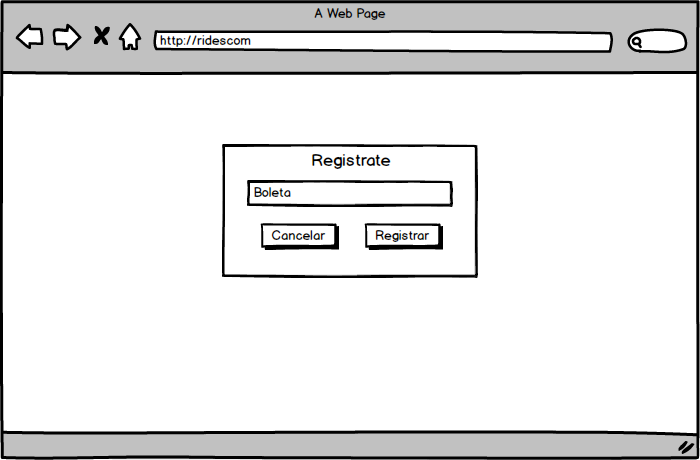
\includegraphics[width=10cm, height=6cm]{Imagenes/Disenos/VistasBorradas/p1_Registro.png}
	\caption{Registro para los alumnos.}
\end{figure}

\begin{figure}[hbt!]
	\centering
	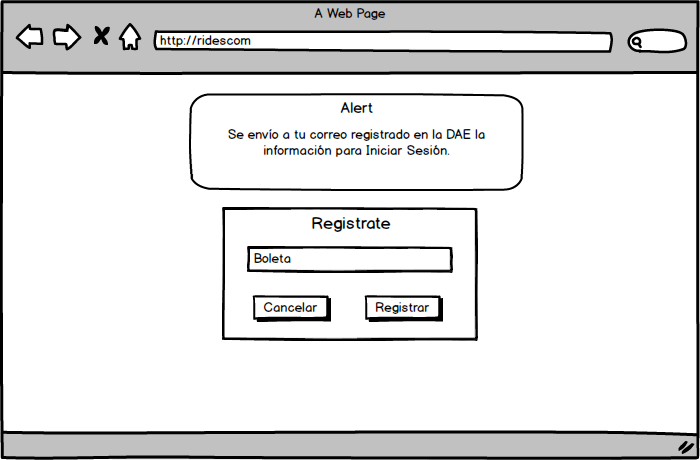
\includegraphics[width=10cm, height=6cm]{Imagenes/Disenos/VistasBorradas/ConfirmacionRegistro.png}
	\caption{Confirmación registro para los alumnos.}
\end{figure}

\begin{figure}[hbt!]
	\centering
	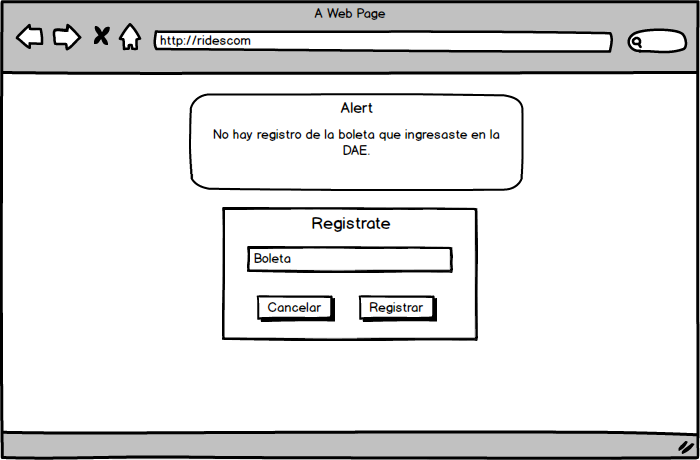
\includegraphics[width=10cm, height=6cm]{Imagenes/Disenos/VistasBorradas/p3RechazoRegistro.png}
	\caption{Rechazo registro para los alumnos.}
\end{figure}

\begin{figure}[hbt!]
	\centering
	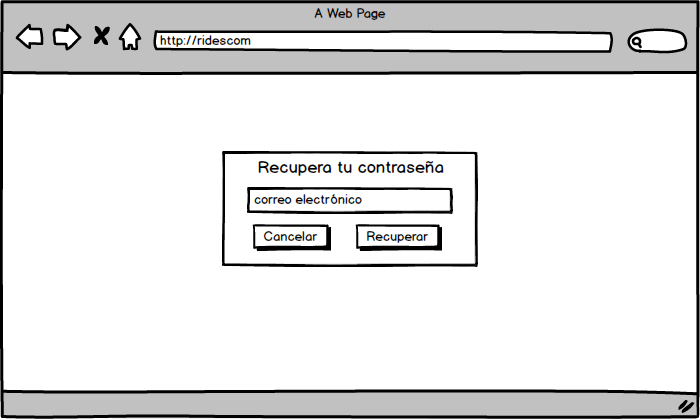
\includegraphics[width=10cm, height=6cm]{Imagenes/Disenos/VistasBorradas/p5Recuperarcontrasena.png}
	\caption{Recuperar contraseña para los alumnos.}
\end{figure}

\begin{figure}[hbt!]
	\centering
	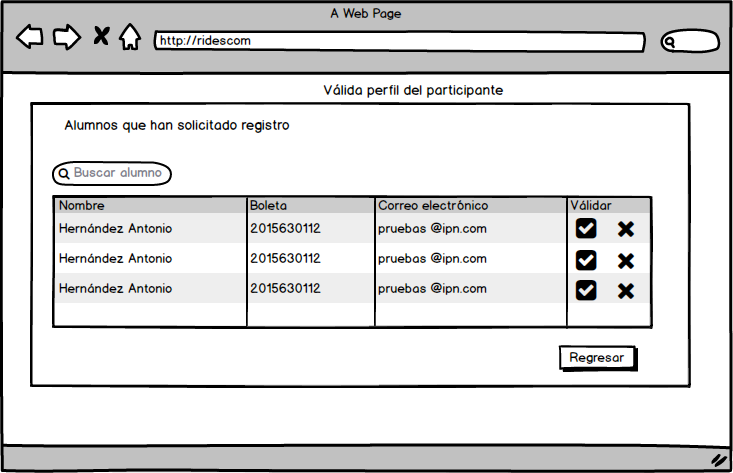
\includegraphics[width=10cm, height=6cm]{Imagenes/Disenos/VistasBorradas/p18ValidaPerfil.png}
	\caption{Validar perfil de los alumnos.}
\end{figure}
\pagebreak

